\documentclass{beamer}

\usetheme{UiO}

\usepackage{array}
\usepackage{pgfplots}
\usepackage{pgfplotstable}

\usepgfplotslibrary{fillbetween}

\usetikzlibrary{arrows}
\usetikzlibrary{arrows.meta}
\usetikzlibrary{positioning}

\title{Exploring the brain with explainable artificial intelligence}
\subtitle{Characterizing diversity in patients with dementia}
\author{Esten H. Leonardsen}
\date{\today}

\definecolor{cases-default}{HTML}{DD0000}
\definecolor{controls-default}{HTML}{006EDB}
\definecolor{healthy-default}{HTML}{09D31D}
\definecolor{additional}{HTML}{A21AC1}

\begin{document}
	\begin{frame}
	 	\titlepage
	\end{frame}

    \newcommand{\mriside}[4]{
    \def\mridepth{0.75}

    \node[inner sep=0pt] (input) at (#1, #2) {
        \includegraphics[height=#3, width=#3]{#4}
    };

    \draw[fill=black] (input.north west) --
        ($ (input.north west) + (0.5 * \mridepth, 0.5 * \mridepth) $) --
        ($ (input.north east) + (0.5 * \mridepth, 0.5 * \mridepth) $) --
        (input.north east) -- cycle;
    \draw[fill=black] (input.north east) --
        ($ (input.north east) + (0.5 * \mridepth, 0.5 * \mridepth) $) --
        ($ (input.south east) + (0.5 * \mridepth, 0.5 * \mridepth) $) --
        (input.south east) -- cycle;
    \draw[] (input.north west) --
        ($ (input.north west) - (0.5 * \mridepth, 0.5 * \mridepth) $) --
        ($ (input.south west) - (0.5 * \mridepth, 0.5 * \mridepth) $) --
        (input.south west) -- cycle;
    \draw[] (input.north east) --
        ($ (input.north east) - (0.5 * \mridepth, 0.5 * \mridepth) $) --
        ($ (input.south east) - (0.5 * \mridepth, 0.5 * \mridepth) $) --
        (input.south east) -- cycle;
    \draw[] ($ (input.north west) - (0.5 * \mridepth, 0.5 * \mridepth) $) --
        ($ (input.north east) - (0.5 * \mridepth, 0.5 * \mridepth) $);
    \draw[] ($ (input.south west) - (0.5 * \mridepth, 0.5 * \mridepth) $) --
        ($ (input.south east) - (0.5 * \mridepth, 0.5 * \mridepth) $);
}


\newcommand{\inputside}[3]{
    \mriside{#1}{#2}{#3}{data/mri_sagittal.png}
}

\newcommand{\heatmapside}[3]{
    \mriside{#1}{#2}{#3}{data/combined_sagittal.png}
}

\newcommand{\convside}[6]{
    \def\sidex{#1}
    \def\sidey{#2}
    \def\sidewidth{#3}
    \def\sideheight{#4}
    \def\sidefillcolour{#5}
    \def\sidename{#6}

    \node[
        fill=\sidefillcolour,
        inner sep=0pt,
        outer sep=0pt,
        minimum width=\sidewidth,
        minimum height=\sideheight,
        draw=black
    ] (\sidename) at (\sidex, \sidey) {};
}

\newcommand{\convtop}[4]{
    \def\topbase{#1}
    \def\topwidth{#2}
    \def\topheight{#3}
    \def\topfillcolour{#4}

    \draw[fill=\topfillcolour,draw=black] #1 --
        ($ #1 + (#3, #3) $) --
        ($ #1 + (#3+#2, #3) $) --
        ($ #1 + (#2, 0) $);
}

\newcommand{\convfront}[3]{
    \def\frontbase{#1}
    \def\frontsize{#2}
    \def\frontfillcolour{#3}

    \draw[black, fill=\frontfillcolour] #1 --
        ($ #1 + (1*#2, 1*#2) $) --
        ($ #1 + (1*#2, 1*#2 - 2*#2) $) --
        ($ #1 + (0, -2*#2) $);
}

\newcommand{\convchannel}[7]{
    \def\channelx{#1}
    \def\channely{#2}
    \def\channelnodedepth{#3}
    \def\channelnodesize{#4}
    \def\channelnodecount{#5}
    \def\channelcolour{#6}
    \def\includefront{#7}

    \def\huemin{20}
    \def\huemax{80}

    \pgfmathsetmacro{\iterations}{#5-1}
    \foreach \i in {0,...,\iterations} {
        \pgfmathsetmacro{\hue}{int(random(\huemin, \huemax))}
        \convside{#1}{#2+\i*-#4}{#3 cm}{#4 cm}{#6!\hue}{n\i0}

        \foreach \j in {0,...,\iterations} {
            \pgfmathsetmacro{\innerhue}{int(random(\huemin, \huemax))}
            \ifnum\j=0
                \pgfmathsetmacro{\innerhue}{\hue}
            \fi

            \ifnum\includefront=1
                \convfront{($ (n00.north east) + (0.5*\j*#4, 0.5*\j*#4 - \i*#4) $)}{0.5*#4}{#6!\innerhue}
            \fi

            \ifnum\i=0
                \convtop{($ (n\i0.north west) + (0.5*\j*#4, 0.5*\j*#4) $)}{#3}{0.5*#4}{#6!\innerhue}
            \fi
        }
    }
}
\newcommand{\lrpchannel}[6]{
    \def\channelx{#1}
    \def\channely{#2}
    \def\channelnodedepth{#3}
    \def\channelnodesize{#4}
    \def\channelnodecount{#5}
    \def\includefront{#6}

    \colorlet{bgcolour}{black!85}

    \pgfmathsetmacro{\iterations}{#5-1}
    \foreach \i in {0,...,\iterations} {
        \pgfmathsetmacro{\hue}{int(random(-150, 100))}
        \colorlet{fillcolour}{bgcolour}

        \colorlet{lrpcolour}{red}
        \pgfmathsetmacro{\coinflip}{int(random(0, 1))}

        \ifnum\coinflip=1
            \colorlet{lrpcolour}{blue}
        \fi

        \ifnum\hue>0
            \colorlet{fillcolour}{lrpcolour!\hue!bgcolour}
        \fi

        \convside{#1}{#2+\i*-#4}{#3 cm}{#4 cm}{fillcolour}{n\i0}

        \foreach \j in {0,...,\iterations} {
            \pgfmathsetmacro{\innerhue}{int(random(-150, 100))}
            \colorlet{innerfillcolour}{bgcolour}

            \ifnum\innerhue>0
                \colorlet{innerfillcolour}{lrpcolour!\innerhue!bgcolour}
            \fi

            \ifnum\j=0
                \colorlet{innerfillcolour}{fillcolour}
            \fi

            \ifnum\includefront=1
                \convfront{($ (n00.north east) + (0.5*\j*#4, 0.5*\j*#4 - \i*#4) $)}{0.5*#4}{innerfillcolour}
            \fi

            \ifnum\i=0
                \convtop{($ (n\i0.north west) + (0.5*\j*#4, 0.5*\j*#4) $)}{#3}{0.5*#4}{innerfillcolour}
            \fi
        }
    }
}


\newcommand{\convlayer}[7]{
    \def\layerx{#1}
    \def\layery{#2}
    \def\layernodedepth{#3}
    \def\layernodesize{#4}
    \def\layernodecount{#5}
    \def\layerdepth{#6}
    \def\layercolour{#7}

    \pgfmathsetmacro{\layeriterations}{\layerdepth-1}
    \foreach \i in {0,...,\layeriterations}{
        \pgfmathsetmacro{\x}{\layerx + \i * \layernodedepth}
        \pgfmathsetmacro{\islast}{\i == \layeriterations ? 1 : 0}
        \convchannel{\x}{\layery}{\layernodedepth}{\layernodesize}{\layernodecount}{\layercolour}{\islast}
    }
}
\newcommand{\lrplayer}[6]{
    \def\layerx{#1}
    \def\layery{#2}
    \def\layernodedepth{#3}
    \def\layernodesize{#4}
    \def\layernodecount{#5}
    \def\layerdepth{#6}

    \pgfmathsetmacro{\layeriterations}{\layerdepth-1}
    \foreach \i in {0,...,\layeriterations}{
        \pgfmathsetmacro{\x}{\layerx + \i * \layernodedepth}
        \pgfmathsetmacro{\islast}{\i == \layeriterations ? 1 : 0}
        \lrpchannel{\x}{\layery}{\layernodedepth}{\layernodesize}{\layernodecount}{\islast}
    }
}

\newcommand{\modelarrow}[5]{
    \begin{scope}[transparency group, opacity=0.5]
        \draw[-stealth, line width=2pt, #3] #1 to [in=#4, out=#5] #2;
    \end{scope}
}
\newcommand{\cnnarrow}[3]{
    \modelarrow{#1}{#2}{#3}{180}{0}
}
\newcommand{\lrparrow}[3]{
    \modelarrow{#1}{#2}{#3}{0}{180}
}

\newcommand{\cnn}[6]{
    \def\xmin{#1}
    \def\ymin{#2}
    \def\nodedepth{#3}
    \def\nodesize{#4}
    \def\modelcolour{#5}
    \def\annotate{#6}

    \convlayer{#1 - 0.06 + 0.4}{#2 + 2.5 * #4}{#3}{#4}{12}{3}{\modelcolour}
    \cnnarrow{(#1 + 1.04, #2)}{(#1+2.2, #2)}{black}

    \convlayer{#1 + 1.44 + 0.4}{#2 + 1.5 * #4}{#3}{#4}{8}{5}{\modelcolour}
    \cnnarrow{(#1 + 2.59, #2)}{(#1+3.5, #2)}{black}

    \convlayer{#1 + 2.77 + 0.4}{#2 + 0.5 * #4}{#3}{#4}{4}{7}{\modelcolour}
    \cnnarrow{(#1 + 3.98, #2)}{(#1+5, #2)}{black}

    \convlayer{#1 + 3.93 + 0.4}{#2 + 0}{#3}{#4}{2}{9}{\modelcolour}

    \draw[thick, dashed] (#1 + 0.22, #2 + 1.43) --
                        (#1 + 5.4, #2 + 1.43) --
                        (#1 + 5.4, #2 - 1.42) --
                        (#1 + 0.22, #2 - 1.42) -- cycle;
    \node[anchor=south, text depth=0, font=\footnotesize\selectfont] at (#1 + 2.675, #2 + 1.43) {
        \textbf{Convolutional neural network}
    };
}
\newcommand{\lrp}[4]{
    \def\xmin{#1}
    \def\ymin{#2}
    \def\nodedepth{#3}
    \def\nodesize{#4}

    \lrplayer{#1 - 0.06 + 0.4}{#2 + 2.5 * #4}{#3}{#4}{12}{3}{black}
    \lrparrow{(#1+2.2, #2)}{(#1 + 1.04, #2)}{black}

    \lrplayer{#1 + 1.44 + 0.4}{#2 + 1.5 * #4}{#3}{#4}{8}{5}{black}
    \lrparrow{(#1+3.5, #2)}{(#1 + 2.59, #2)}{black}

    \lrplayer{#1 + 2.77 + 0.4}{#2 + 0.5 * #4}{#3}{#4}{4}{7}{black}
    \lrparrow{(#1+5, #2)}{(#1 + 3.98, #2)}{black}

    \lrplayer{#1 + 3.93 + 0.4}{#2 + 0}{#3}{#4}{2}{9}{black}

    \draw[thick, dashed] (#1 + 0.22, #2 + 1.43) --
                        (#1 + 5.4, #2 + 1.43) --
                        (#1 + 5.4, #2 - 1.42) --
                        (#1 + 0.22, #2 - 1.42) -- cycle;
    \node[anchor=south, text depth=0, font=\footnotesize\selectfont] at (#1 + 2.675, #2 + 1.43) {
        \textbf{Convolutional Neural Network}
    };
}
    \section{Introduction to machine learning}

\begin{frame}{Introduction}
    \begin{tikzpicture}
        \node[] at (-5.25, -3.5) {};
        \node[] at (5.25, 3.5) {};
        \visible<1-3>{
            \node[text width=10.5cm, align=flush left] at (0, 0) {
                \textbf{Key terminology:}
                \begin{itemize}
                    \item Statistical learning: A set of tools (often called models) for finding patterns in data.
                    \item<2-> Machine learning: Approximately the same as statistical learning.
                    \begin{itemize}
                        \item<2-> More common among practitioners with a computer science or engineering background.
                        \item<2-> Often has a focus on prediction (as opposed to understanding).
                        \item<2-> Often uses very large datasets.
                        \item<2-> More pragmatic in nature(?).
                    \end{itemize}
                    \item<3> Supervised learning: We know what task we want the model to solve.
                    \item<3> Unsupervised learning: We don't know what task we want the model to solve (or we don't have the data needed to solve it).
                \end{itemize}
            };
        }
        \visible<4-5,7-8>{

            \node[inner sep=0pt, draw=black, anchor=west] (x1) at (-5.25, 2.5) {
                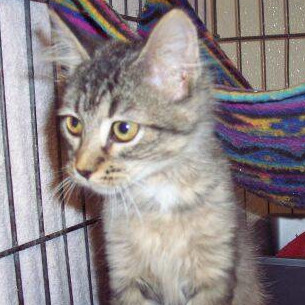
\includegraphics[width=1cm]{data/cats_and_dogs/cat.2.jpg}
            };
            \node[inner sep=0pt, draw=black] (x2) at ($ (x1) - (0, 1.5) $) {
                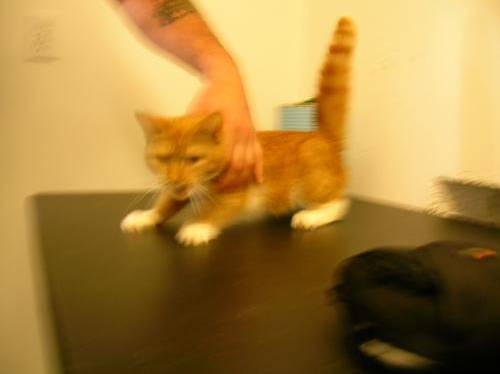
\includegraphics[width=1cm]{data/cats_and_dogs/cat.0.jpg}
            };
            \node[inner sep=0pt, draw=black] (x3) at ($ (x1) - (0, 3) $) {
                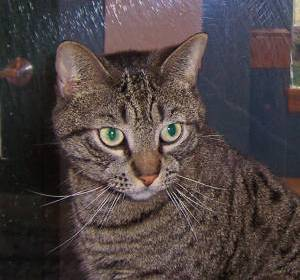
\includegraphics[width=1cm]{data/cats_and_dogs/cat.1.jpg}
            };
            \node[inner sep=0pt, draw=black] (x3) at ($ (x1) - (0, 4.5) $) {
                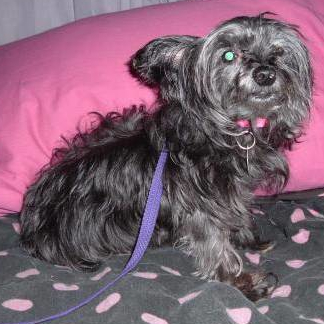
\includegraphics[width=1cm]{data/cats_and_dogs/dog.0.jpg}
            };

            \node[inner sep=0pt, draw=black] (x5) at ($ (x1) - (-1.25, 0.75) $) {
                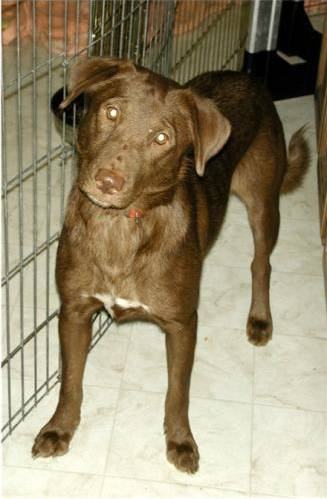
\includegraphics[width=1cm]{data/cats_and_dogs/dog.1.jpg}
            };
            \node[inner sep=0pt, draw=black] (x6) at ($ (x1) - (-1.25, 2.25) $) {
                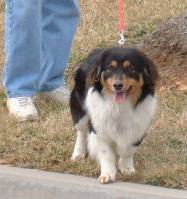
\includegraphics[width=1cm]{data/cats_and_dogs/dog.2.jpg}
            };
            \node[inner sep=0pt, draw=black] (x7) at ($ (x1) - (-1.25, 3.75) $) {
                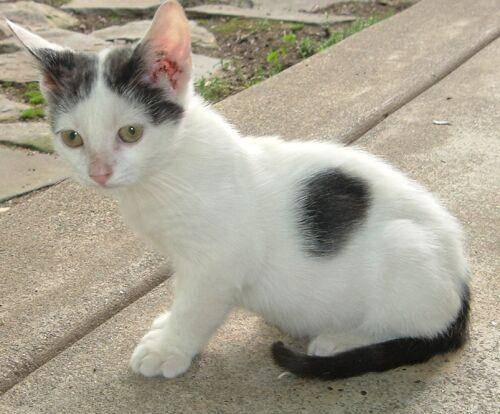
\includegraphics[width=1cm]{data/cats_and_dogs/cat.3.jpg}
            };
        }
        \visible<6>{
            \node[inner sep=0pt, draw=black, anchor=west, label=below:\tiny{Cat}] (x1) at (-5.25, 2.5) {
                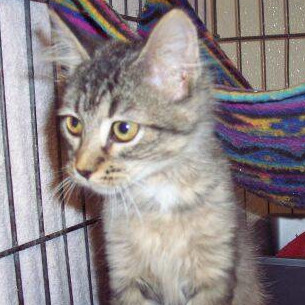
\includegraphics[width=1cm]{data/cats_and_dogs/cat.2.jpg}
            };
            \node[inner sep=0pt, draw=black, label=below:\tiny{Cat}] (x2) at ($ (x1) - (0, 1.5) $) {
                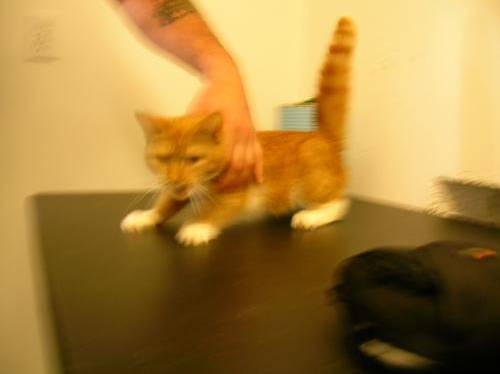
\includegraphics[width=1cm]{data/cats_and_dogs/cat.0.jpg}
            };
            \node[inner sep=0pt, draw=black, label=below:\tiny{Cat}] (x3) at ($ (x1) - (0, 3) $) {
                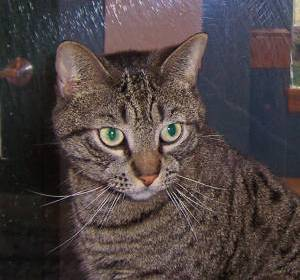
\includegraphics[width=1cm]{data/cats_and_dogs/cat.1.jpg}
            };
            \node[inner sep=0pt, draw=black, label=below:\tiny{Dog}] (x3) at ($ (x1) - (0, 4.5) $) {
                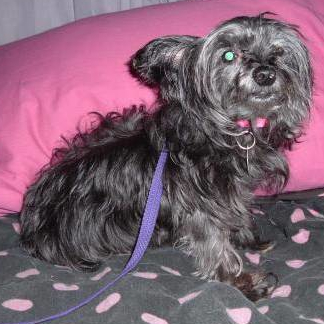
\includegraphics[width=1cm]{data/cats_and_dogs/dog.0.jpg}
            };

            \node[inner sep=0pt, draw=black, label=below:\tiny{Dog}] (x5) at ($ (x1) - (-1.25, 0.75) $) {
                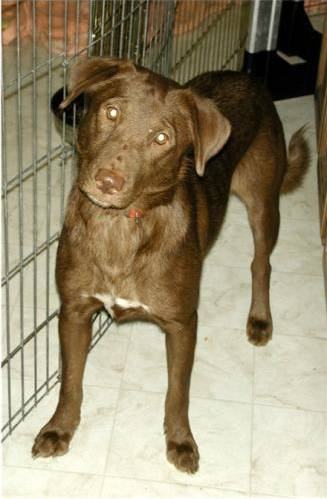
\includegraphics[width=1cm]{data/cats_and_dogs/dog.1.jpg}
            };
            \node[inner sep=0pt, draw=black, label=below:\tiny{Dog}] (x6) at ($ (x1) - (-1.25, 2.25) $) {
                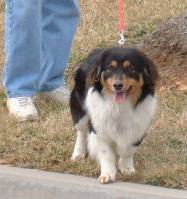
\includegraphics[width=1cm]{data/cats_and_dogs/dog.2.jpg}
            };
            \node[inner sep=0pt, draw=black, label=below:\tiny{Cat}] (x7) at ($ (x1) - (-1.25, 3.75) $) {
                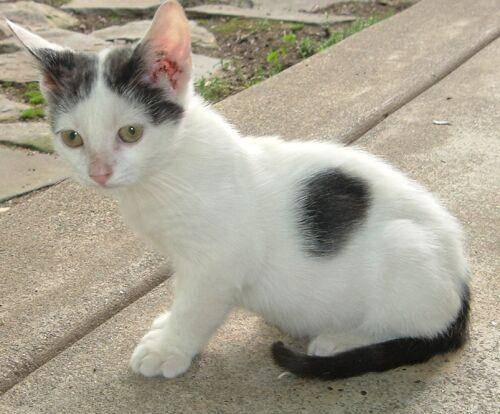
\includegraphics[width=1cm]{data/cats_and_dogs/cat.3.jpg}
            };
        }
        \visible<5-6,9>{
            \node[align=center, font=\scriptsize, draw=black] (sm) at ($ (x1) + (3.5, -0.75) $) {
                Supervised\\model
            };
        }
        \visible<5-6>{
            \draw[-stealth, gray!50, line width=3pt] (x6) to [in=270, out=0] (sm);
            \draw[-stealth, gray!50, line width=3pt] (sm) -- ($ (sm.east) + (1.1, 0) $);

            \node[inner sep=0pt, draw=black] (y1) at ($ (sm.center) + (5, 0.5) $) {
                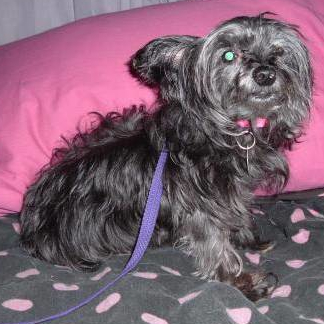
\includegraphics[width=1cm]{data/cats_and_dogs/dog.0.jpg}
            };
            \node[anchor=west, inner sep=0pt, draw=black] (y2) at (y1.east) {
                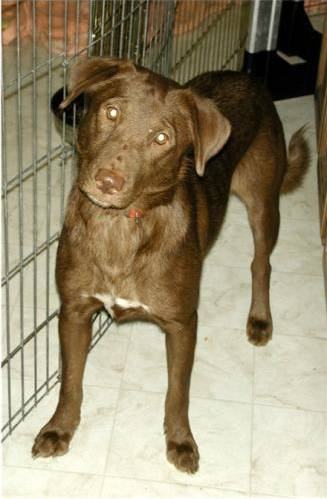
\includegraphics[width=1cm]{data/cats_and_dogs/dog.1.jpg}
            };
            \node[anchor=north, inner sep=0pt, draw=black] at (y1.south) {
                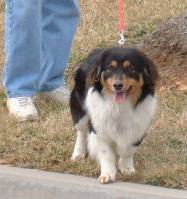
\includegraphics[width=1cm]{data/cats_and_dogs/dog.2.jpg}
            };

            \node[inner sep=0pt, draw=black] (y4) at ($ (sm) + (2.5, 0.5) $) {
                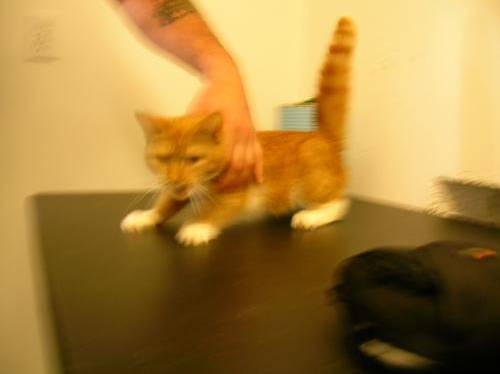
\includegraphics[width=1cm]{data/cats_and_dogs/cat.0.jpg}
            };
            \node[anchor=west, inner sep=0pt, draw=black] (y5) at (y4.east) {
                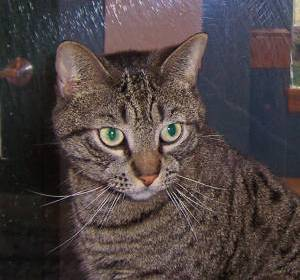
\includegraphics[width=1cm]{data/cats_and_dogs/cat.1.jpg}
            };
            \node[anchor=north, inner sep=0pt, draw=black] (y6) at (y4.south) {
                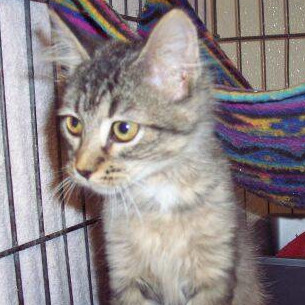
\includegraphics[width=1cm]{data/cats_and_dogs/cat.2.jpg}
            };
            \node[anchor=north, inner sep=0pt, draw=black] (y7) at (y5.south) {
                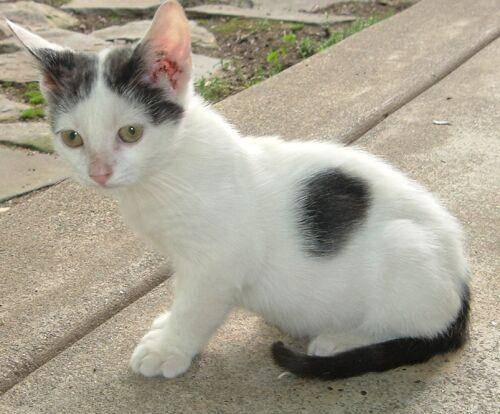
\includegraphics[width=1cm]{data/cats_and_dogs/cat.3.jpg}
            };

            \node[anchor=south, text depth=0] at ($ (y1.north)!0.5!(y2.north) $) {
                Dogs
            };
            \node[anchor=south, text depth=0] at ($ (y4.north)!0.5!(y5.north) $) {
                Cats
            };
        }
        \visible<7-9>{
            \node[align=center, font=\scriptsize, draw=black] (um) at ($ (x1) + (3.5, -3.75) $) {
                Unsupervised\\model
            };
        }
        \visible<7-8>{

            \draw[-stealth, gray!50, line width=3pt] (x6) to [in=90, out=0] (um);
            \draw[-stealth, gray!50, line width=3pt] (um) -- ($ (um.east) + (1.1, 0) $);
        }
        \visible<7>{
            \node[inner sep=0pt, draw=black] at ($ (um.center) + (6, 0.55) $) {
                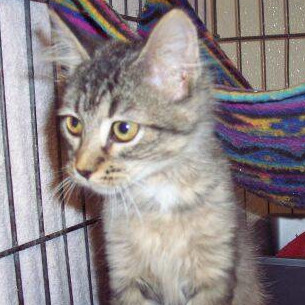
\includegraphics[width=1cm]{data/cats_and_dogs/cat.2.jpg}
            };
            \node[inner sep=0pt, draw=black] at ($ (um.center) + (5.95, -0.65) $) {
                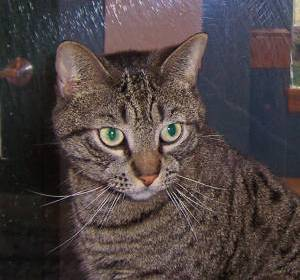
\includegraphics[width=1cm]{data/cats_and_dogs/cat.1.jpg}
            };
            \node[inner sep=0pt, draw=black] at ($ (um.center) + (4.8, 0.4) $) {
                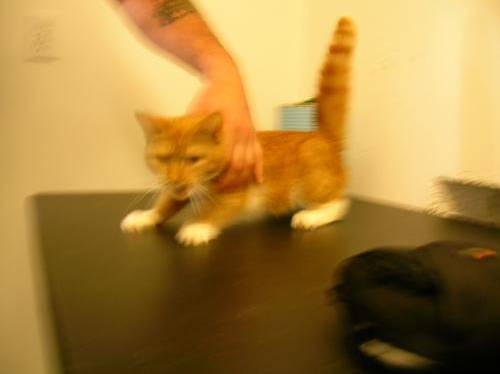
\includegraphics[width=1cm]{data/cats_and_dogs/cat.0.jpg}
            };
            \node[inner sep=0pt, draw=black] at ($ (um.center) + (4.7, -0.7) $) {
                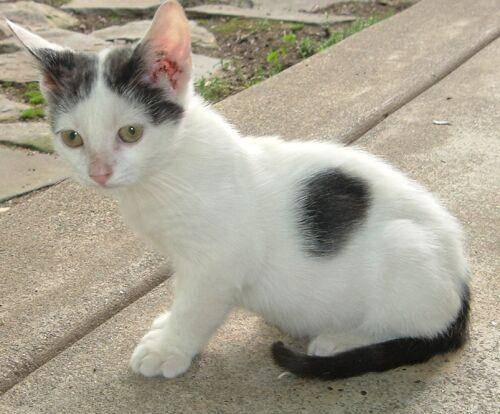
\includegraphics[width=1cm]{data/cats_and_dogs/cat.3.jpg}
            };

            \node[inner sep=0pt, draw=black] at ($ (um.center) + (2.7, 1.2) $) {
                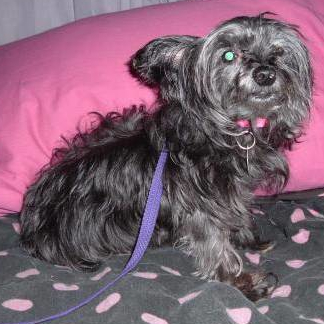
\includegraphics[width=1cm]{data/cats_and_dogs/dog.0.jpg}
            };
            \node[inner sep=0pt, draw=black] at ($ (um.center) + (2.55, 0) $) {
                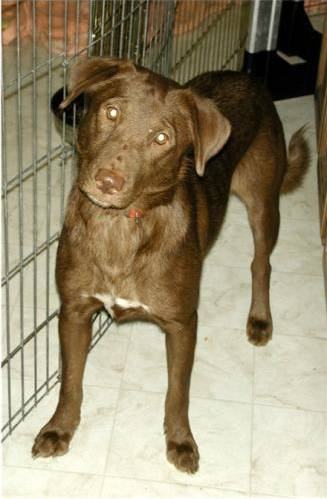
\includegraphics[width=1cm]{data/cats_and_dogs/dog.1.jpg}
            };
            \node[inner sep=0pt, draw=black] at ($ (um.center) + (2.65, -1.1) $) {
                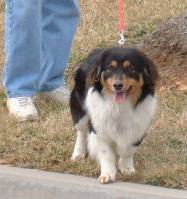
\includegraphics[width=1cm]{data/cats_and_dogs/dog.2.jpg}
            };
        }
        \visible<8>{
            \node[inner sep=0pt, draw=black] at ($ (um.center) + (6, 0.55) $) {
                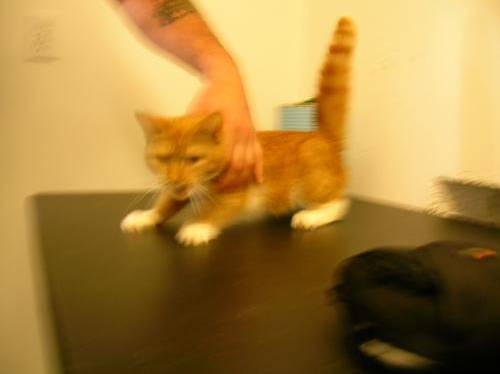
\includegraphics[width=1cm]{data/cats_and_dogs/cat.0.jpg}
            };
            \node[inner sep=0pt, draw=black] at ($ (um.center) + (5.95, -0.65) $) {
                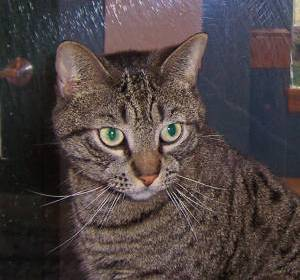
\includegraphics[width=1cm]{data/cats_and_dogs/cat.1.jpg}
            };
            \node[inner sep=0pt, draw=black] at ($ (um.center) + (4.8, 0.4) $) {
                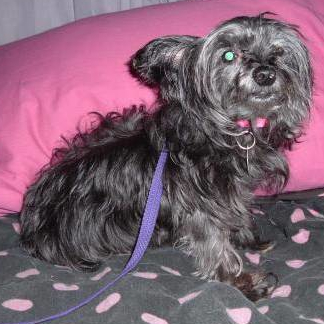
\includegraphics[width=1cm]{data/cats_and_dogs/dog.0.jpg}
            };
            \node[inner sep=0pt, draw=black] at ($ (um.center) + (4.7, -0.7) $) {
                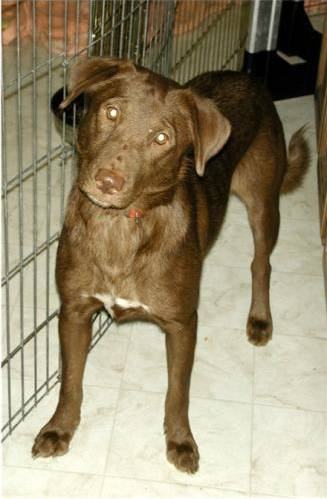
\includegraphics[width=1cm]{data/cats_and_dogs/dog.1.jpg}
            };

            \node[inner sep=0pt, draw=black] at ($ (um.center) + (2.7, 1.2) $) {
                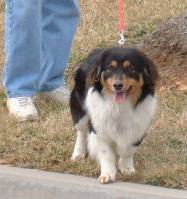
\includegraphics[width=1cm]{data/cats_and_dogs/dog.2.jpg}
            };
            \node[inner sep=0pt, draw=black] at ($ (um.center) + (2.55, 0) $) {
                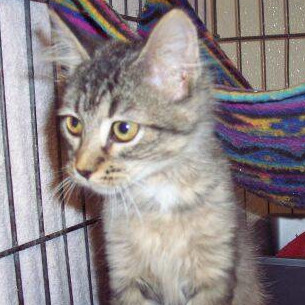
\includegraphics[width=1cm]{data/cats_and_dogs/cat.2.jpg}
            };
            \node[inner sep=0pt, draw=black] at ($ (um.center) + (2.65, -1.1) $) {
                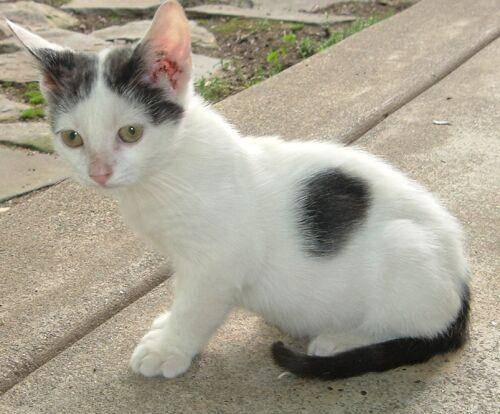
\includegraphics[width=1cm]{data/cats_and_dogs/cat.3.jpg}
            };
        }

    \end{tikzpicture}
\end{frame}

\newcommand{\mpgvsweight}[1]{
    \begin{tikzpicture}
        \begin{axis}[
            height=4cm,
            width=10cm,
            xlabel=$x$ (horsepower),
            ylabel=$y$ (mpg),
            ytick pos=left,
            xtick pos=bottom,
            xmin=30,
            xmax=245,
            ymin=6,
            ymax=51
        ]

        \addplot[
            only marks,
            cyan,
            opacity=0.5
        ] table [
            col sep=comma,
            x=horsepower,
            y=mpg
        ] {data/Auto.csv};

        \ifnum#1=1
            \draw[very thick, red] (axis cs: 30, 39-0.157*30) -- (axis cs: 245, 39-0.157*245);
            \node[text=red] at (axis cs: 180, 42) {
                $\hat{f}(x) = 39 - 0.157x$
            };
        \fi
        \ifnum#1=2
            \addplot[very thick, red, domain=30:245, samples=1000] {0.0012*x^2-0.46*x+56};
            \node[text=red] at (axis cs: 180, 42) {
                $\hat{f}(x) = 56+0.0012x^2-0.46x$
            };
        \fi
        \ifnum#1=3
            \addplot[very thick, red, smooth] coordinates {
                (6.0, 243.2069751806266)
                (15.958333333333334, 118.86132183998052)
                (25.916666666666668, 55.54830308937471)
                (35.875, 33.03657403682814)
                (45.833333333333336, 31.094789790600284)
                (55.79166666666667, 32.62203312809545)
                (65.75, 32.322995894942245)
                (75.70833333333334, 26.789726618159705)
                (85.66666666666667, 25.56443372228785)
                (95.625, 23.411114113578773)
                (105.58333333333334, 21.972291293527256)
                (115.54166666666667, 22.0202279029072)
                (125.5, 19.623191768387127)
                (135.45833333333334, 17.796535374305538)
                (145.41666666666669, 15.42464063855285)
                (155.375, 13.83975395598323)
                (165.33333333333334, 13.58266973340266)
                (175.29166666666669, 14.577234897250934)
                (185.25, 13.44873671948327)
                (195.20833333333334, 11.13569858732588)
                (205.16666666666669, 10.948027264126887)
                (215.125, 12.746078206932541)
                (225.08333333333334, 14.710541046885707)
                (235.04166666666669, 16.775438769652766)
                (245.0, 18.301538120974897)
            };
            \node[text=red] at (axis cs: 180, 42) {
                $\hat{f}(x) = \ldots$
            };
        \fi
        \ifnum#1>3
            \draw[very thick, red] (axis cs: 30, 39-0.157*30) -- (axis cs: 245, 39-0.157*245);
        \fi
        \ifnum#1=4
            \node[minimum height=0.4cm, minimum width=1.15cm, draw=black, very thick] at (axis cs: 197, 42) {};

            \node[text=red] at (axis cs: 180, 42) {
                $\hat{f}(x) = 39 - 0.157x$
            };
        \fi
        \ifnum#1>4
            \addplot[
                only marks,
                red,
                opacity=0.5
            ] coordinates {
                (125, 19.3)
            };
            \node[text=red, anchor=north] at (axis cs: 180, 48.4) {
                $\begin{aligned}
                \hat{f}(125) &= 39 - 0.157*125\\[-0.25cm]
                &= 19.3
                \end{aligned}$
            };
        \fi
        \ifnum#1>5
            \node[text=red] (yhat) at (axis cs: 176.5, 22) {
                $\hat{y}$
            };
            \draw[-stealth, red] (yhat.north) -- ($ (yhat.north) +( 0, 50) $);
        \fi

        \end{axis}
    \end{tikzpicture}
}

\newsavebox{\mpgpoints}
\sbox{\mpgpoints}{
    \mpgvsweight{0}
}
\newsavebox{\mpglinear}
\sbox{\mpglinear}{
    \mpgvsweight{1}
}
\newsavebox{\mpgsquared}
\sbox{\mpgsquared}{
    \mpgvsweight{2}
}
\newsavebox{\mpgnonparametric}
\sbox{\mpgnonparametric}{
    \mpgvsweight{3}
}
\newsavebox{\mpglinearhighlight}
\sbox{\mpglinearhighlight}{
    \mpgvsweight{4}
}
\newsavebox{\mpgcalculation}
\sbox{\mpgcalculation}{
    \mpgvsweight{5}
}
\newsavebox{\mpgyhat}
\sbox{\mpgyhat}{
    \mpgvsweight{6}
}

\begin{frame}{Introduction: Supervised learning}
    \begin{tikzpicture}
        \node[] at (-5.25, -3.5) {};
        \node[] at (5.25, 3.5) {};

        \visible<1-5>{
            \node[anchor=north west, ampersand replacement=\&, font=\footnotesize] at (-5.25, 3.5) {
                \begin{tabular}{|c|c|c|c|c|c|}
                    \hline
                    \textbf{name}&\alert<4>{\textbf{year}}&\alert<4>{\textbf{cylinders}}&\alert<4>{\textbf{horsepower}}&\alert<4>{\textbf{weight}}&\alert<3>{\textbf{mpg}}\\
                    \hline
                    Chevrolet Chevelle Malibu&\alert<4>{1970}&\alert<4>{8}&\alert<4>{130}&\alert<4>{3504}&\alert<3>{18}\\
                    \alert<2>{Buick Skylark 320}&\alert<2,4>{1980}&\alert<2,4>{4}&\alert<2,4>{165}&\alert<2,4>{3693}&\alert<2,3>{15}\\
                    Plymouth Satellite&\alert<4>{1971}&\alert<4>{8}&\alert<4>{150}&\alert<4>{3436}&\alert<3>{18}\\
                    AMC Rebel SST&\alert<4>{1975}&\alert<4>{4}&\alert<4>{150}&\alert<4>{3433}&\alert<3>{16}\\
                    Ford Torino&\alert<4>{1978}&\alert<4>{8}&\alert<4>{140}&\alert<4>{3449}&\alert<3>{17}\\
                    \hline
                \end{tabular}
            };
            \node[anchor=south west, text width=10.5cm] at (-5.25, -3.5) {
                \textbf{Prerequisites}
                \begin{itemize}
                    \item A dataset representing a given population
                    \item<3-> A response-variable $y$ that we want to predict
                    \item<4-> A set of predictors $X$ that we can use to predict $y$
                    \item<5-> An \textbf{assumed} relationship between $X$ and $y$ that can be described by an unknown function $f$, such that $y=f(X) + \epsilon$
                \end{itemize}
            };
        }
        \visible<6>{
            \node[] at (0, 1.75) {
                \usebox{\mpgpoints}
            };
        }
        \visible<7,9,11,13,15>{
            \node[] at (0, 1.75) {
                \usebox{\mpglinear}
            };
        }
        \visible<8,14>{
            \node[] at (0, 1.75) {
                \usebox{\mpgsquared}
            };
        }
        \visible<10>{
            \node[] at (0, 1.75) {
                \usebox{\mpgnonparametric}
            };
        }
        \visible<6-10>{
            \node[anchor=north west, text width=10.5cm] at (-5.25, 0) {
                \textbf{Estimation (or training the model)}
                \begin{itemize}
                    \item We have assumed that $y=f(X) + \epsilon$, but don't know $f$
                    \item<7-> We produce an estimate $\hat{f}$
                    \item<9-> Parametric models: $\hat{f}$ has a simple form
                    \begin{itemize}
                        \item<9-> $\hat{f}(x) = {\color{red}\beta_0} + {\color{red}\beta_1} x$
                    \end{itemize}
                    \item<10-> Non-parametric models: $\hat{f}$ relies directly on the data
                \end{itemize}
            };
        }
        \visible<12>{
           \node[] at (0, 1.75) {
               \usebox{\mpglinearhighlight}
           };
        }
        \visible<11-17>{
            \node[anchor=north west, text width=10.5cm, align=flush left] (inference) at (-5.25, 0) {
                \textbf{Inference: Understanding the relationship between the predictors and the response}
                \begin{itemize}
                    \item<12-> How does individual features relate to the response?
                    \item<13-> What is the \textit{functional form} of the relationship?
                \end{itemize}
            };
        }
        \visible<15-17>{
            \node[anchor=north west, text width=10.5cm, align=flush left] at (inference.south west) {
                \textbf{Prediction: Predicting the response for new observations}
                \begin{itemize}
                    \item Plugging new values $X$ into $\hat{f}(X)$
                \end{itemize}
            };
        }
        \visible<16>{
            \node[] at (0, 1.75) {
                \usebox{\mpgcalculation}
            };
        }
        \visible<17>{
            \node[] at (0, 1.75) {
                \usebox{\mpgyhat}
            };
        }
        \visible<18>{
            \node[] at (0, 0) {
                \url{http://localhost:8888/tree}
            };
        }
    \end{tikzpicture}
\end{frame}

\begin{frame}{Introduction: Functional interfaces}
    \begin{tikzpicture}
        \node[] at (-5.25, -3.5) {};
        \node[] at (5.25, 3.5) {};

        \visible<1-4>{
            \node[draw=black, fill=gray!20, minimum height=0.6cm, rounded corners=0.1cm] (prep) at (-3.3, 2) {
                Preparations
            };
            \node[draw=black, fill=gray!20, minimum height=0.6cm, rounded corners=0.1cm, anchor=west] (train) at ($ (prep.east) + (0.5, 0) $) {
                Model training
            };
            \node[draw=black, fill=gray!20, minimum height=0.6cm, rounded corners=0.1cm, anchor=west] (eval) at ($ (train.east) + (0.5, 0) $) {
                Model application
            };
            \draw[-stealth] (prep) -- (train);
            \draw[-stealth] (train) -- (eval);
        }
        \visible<2-4>{
            \node[draw=black, fill=blue!80, font=\footnotesize, text=white, rounded corners=0.1cm, text depth=1cm, minimum width=2cm] (linear) at ($ (train.south east)!0.5!(eval.south west) - (0, 1.5) $) {
                Linear
            };
            \draw[thick, white] ($ (linear.south west) + (0.2, 0.2) $) -- ($ (linear.south east) + (-0.2, 0.8) $);

            \draw[dashed, -stealth] (linear.north) |- ($ (train.south) - (0, 0.4) $) -| (train.south);
            \draw[dashed, -stealth] (linear.north) |- ($ (eval.south) - (0, 0.4) $) -| (eval.south);
        }
        \visible<3-4>{
            \node[draw=black, fill=blue!80, font=\footnotesize, text=white, rounded corners=0.1cm, text depth=1cm, minimum width=2cm] (trees) at ($ (train.south east)!0.5!(eval.south west) - (0, 3.5) $) {
                Trees
            };
            \node[circle, draw=white, thick, inner sep=2pt] (t0) at ($ (trees) + (0, 0.1) $) {};
            \node[circle, draw=white, thick, inner sep=2pt] (t1) at ($ (trees) + (0.3, -0.4) $) {};
            \node[circle, draw=white, thick, inner sep=2pt] (t2) at ($ (trees) + (-0.3, -0.4) $) {};
            \draw[thick, white] (t0) -- (t1);
            \draw[thick, white] (t0) -- (t2);

            \node[draw=black, fill=blue!80, font=\footnotesize, text=white, rounded corners=0.1cm, text depth=1cm, minimum width=2cm] (nonlinear) at ($ (train.south east)!0.5!(eval.south west) - (-2.5, 1.5) $) {
                Non-linear
            };
            \draw[thick, white] ($ (nonlinear.south west) + (0.2, 0.2) $) to [out=90, in=180] ($ (nonlinear.south east) + (-0.2, 0.8) $);
            \node[draw=black, fill=blue!80, font=\footnotesize, text=white, rounded corners=0.1cm, text depth=1cm, minimum width=2cm] (nn) at ($ (train.south east)!0.5!(eval.south west) - (-2.5, 3.5) $) {
                Neural nets
            };
            \node[circle, draw=white, thick, inner sep=2pt] (n0) at ($ (nn) + (-0.7, 0.1) $) {};
            \node[circle, draw=white, thick, inner sep=2pt] (n1) at ($ (nn) + (-0.7, -0.2) $) {};
            \node[circle, draw=white, thick, inner sep=2pt] (n2) at ($ (nn) + (-0.7, -0.5) $) {};
            \node[circle, draw=white, thick, inner sep=2pt] (n3) at ($ (nn) + (0, -0.05) $) {};
            \node[circle, draw=white, thick, inner sep=2pt] (n4) at ($ (nn) + (0, -0.35) $) {};
            \node[circle, draw=white, thick, inner sep=2pt] (n5) at ($ (nn) + (0.7, -0.2) $) {};

            \draw[thick, white] (n0) -- (n3);
            \draw[thick, white] (n0) -- (n4);
            \draw[thick, white] (n1) -- (n3);
            \draw[thick, white] (n1) -- (n4);
            \draw[thick, white] (n2) -- (n3);
            \draw[thick, white] (n2) -- (n4);
            \draw[thick, white] (n3) -- (n5);
            \draw[thick, white] (n4) -- (n5);

        }
        \visible<4>{
            \node[text width=4.3cm, align=flush left, anchor=north west] at (-4.8, 0.5) {
                \textbf{Functional interface:}\\
                We reason about models based on their high level functionality, not their inner workings
            };
        }
        \visible<5-7>{
            \node[draw=black, fill=blue!80, font=\footnotesize, text=white, rounded corners=0.1cm, text depth=1cm, minimum width=2cm] (linear) at (-4, 2.25) {
                Linear
            };
            \draw[thick, white] ($ (linear.south west) + (0.2, 0.2) $) -- ($ (linear.south east) + (-0.2, 0.8) $);

            \node[draw=black, fill=blue!80, font=\footnotesize, text=white, rounded corners=0.1cm, text depth=1cm, minimum width=2cm] (trees) at (-4, 0.75) {
                Trees
            };
            \node[circle, draw=white, thick, inner sep=2pt] (t0) at ($ (trees) + (0, 0.1) $) {};
            \node[circle, draw=white, thick, inner sep=2pt] (t1) at ($ (trees) + (0.3, -0.4) $) {};
            \node[circle, draw=white, thick, inner sep=2pt] (t2) at ($ (trees) + (-0.3, -0.4) $) {};
            \draw[thick, white] (t0) -- (t1);
            \draw[thick, white] (t0) -- (t2);

            \node[draw=black, fill=blue!80, font=\footnotesize, text=white, rounded corners=0.1cm, text depth=1cm, minimum width=2cm] (nonlinear) at (-4, -0.75) {
                Non-linear
            };
            \draw[thick, white] ($ (nonlinear.south west) + (0.2, 0.2) $) to [out=90, in=180] ($ (nonlinear.south east) + (-0.2, 0.8) $);

            \node[draw=black, fill=blue!80, font=\footnotesize, text=white, rounded corners=0.1cm, text depth=1cm, minimum width=2cm] (nn) at (-4, -2.25) {
                Neural nets
            };
            \node[circle, draw=white, thick, inner sep=2pt] (n0) at ($ (nn) + (-0.7, 0.1) $) {};
            \node[circle, draw=white, thick, inner sep=2pt] (n1) at ($ (nn) + (-0.7, -0.2) $) {};
            \node[circle, draw=white, thick, inner sep=2pt] (n2) at ($ (nn) + (-0.7, -0.5) $) {};
            \node[circle, draw=white, thick, inner sep=2pt] (n3) at ($ (nn) + (0, -0.05) $) {};
            \node[circle, draw=white, thick, inner sep=2pt] (n4) at ($ (nn) + (0, -0.35) $) {};
            \node[circle, draw=white, thick, inner sep=2pt] (n5) at ($ (nn) + (0.7, -0.2) $) {};

            \draw[thick, white] (n0) -- (n3);
            \draw[thick, white] (n0) -- (n4);
            \draw[thick, white] (n1) -- (n3);
            \draw[thick, white] (n1) -- (n4);
            \draw[thick, white] (n2) -- (n3);
            \draw[thick, white] (n2) -- (n4);
            \draw[thick, white] (n3) -- (n5);
            \draw[thick, white] (n4) -- (n5);
        }
        \visible<6>{
            \draw[] ($ (linear.east) + (0, 0.1) $) -- ++(1.3, 0);
            \node[anchor=south west] at ($ (linear.east) + (0, 0.1) $) {Train};
            \draw[] ($ (linear.east) + (0, -0.5) $) -- ++(1.3, 0);
            \node[anchor=south west] at ($ (linear.east) + (0, -0.5) $) {Predict};

            \draw[] ($ (trees.east) + (0, 0.1) $) -- ++(1.3, 0);
            \node[anchor=south west] at ($ (trees.east) + (0, 0.1) $) {Train};
            \draw[] ($ (trees.east) + (0, -0.5) $) -- ++(1.3, 0);
            \node[anchor=south west] at ($ (trees.east) + (0, -0.5) $) {Predict};

            \draw[] ($ (nonlinear.east) + (0, 0.1) $) -- ++(1.3, 0);
            \node[anchor=south west] at ($ (nonlinear.east) + (0, 0.1) $) {Train};
            \draw[] ($ (nonlinear.east) + (0, -0.5) $) -- ++(1.3, 0);
            \node[anchor=south west] at ($ (nonlinear.east) + (0, -0.5) $) {Predict};

            \draw[] ($ (nn.east) + (0, 0.1) $) -- ++(1.3, 0);
            \node[anchor=south west] at ($ (nn.east) + (0, 0.1) $) {Train};
            \draw[] ($ (nn.east) + (0, -0.5) $) -- ++(1.3, 0);
            \node[anchor=south west] at ($ (nn.east) + (0, -0.5) $) {Predict};
        }
        \visible<7>{
            \draw[] ($ (linear.east) + (0, 0.1) $) -- ++(1.7, 0);
            \node[anchor=south west] at ($ (linear.east) + (0, 0.1) $) {fit(X, y)};
            \draw[] ($ (linear.east) + (0, -0.5) $) -- ++(1.7, 0);
            \node[anchor=south west] at ($ (linear.east) + (0, -0.5) $) {predict(X)};

            \draw[] ($ (trees.east) + (0, 0.1) $) -- ++(1.7, 0);
            \node[anchor=south west] at ($ (trees.east) + (0, 0.1) $) {fit(X, y)};
            \draw[] ($ (trees.east) + (0, -0.5) $) -- ++(1.7, 0);
            \node[anchor=south west] at ($ (trees.east) + (0, -0.5) $) {predict(X)};

            \draw[] ($ (nonlinear.east) + (0, 0.1) $) -- ++(1.7, 0);
            \node[anchor=south west] at ($ (nonlinear.east) + (0, 0.1) $) {fit(X, y)};
            \draw[] ($ (nonlinear.east) + (0, -0.5) $) -- ++(1.7, 0);
            \node[anchor=south west] at ($ (nonlinear.east) + (0, -0.5) $) {predict(X)};

            \draw[] ($ (nn.east) + (0, 0.1) $) -- ++(1.7, 0);
            \node[anchor=south west] at ($ (nn.east) + (0, 0.1) $) {fit(X, y)};
            \draw[] ($ (nn.east) + (0, -0.5) $) -- ++(1.7, 0);
            \node[anchor=south west] at ($ (nn.east) + (0, -0.5) $) {predict(X)};
        }
        \visible<8>{
            \node[font=\small] at (0, 0) {
                \url{https://scikit-learn.org/stable/developers/develop.html}
            };
        }
        \visible<9>{
            \node[] at (0, 0) {
                \url{http://localhost:8888/tree}
            };
        }
        \visible<10>{
            \node[text width=10.5cm, align=flush left] at (0, 0) {
                \textbf{Supervised learning: We train a model to solve a problem we already know, and that we already have labels for}\\
                \begin{itemize}
                    \item Although a bunch of things can vary (e.g. how we preprocess the data, the type of model, how we measure performance), the overall pattern very often remains the same:
                    \begin{enumerate}
                        \item Data preparation
                        \item Train the model
                        \item Apply the model
                    \end{enumerate}
                \end{itemize}
            };
        }
    \end{tikzpicture}
\end{frame}

\begin{frame}{Introduction: Model performance}
    \begin{tikzpicture}
        \node[] at (-5.25, -3.5) {};
        \node[] at (5.25, 3.5) {};

        \visible<1-9>{
            \draw[dashed] (0, -3.5) -- (0, 3.5);
        }

        \visible<1-5>{
            \node[anchor=north] at (-2.675, 3.5) {\textbf{Regression}};
        }
        \visible<6-9>{
            \node[anchor=north,text=gray!20] at (-2.675, 3.5) {\textbf{Regression}};
        }
        \visible<1-2,6-9>{
            \node[anchor=north] at (2.675, 3.5) {\textbf{Classification}};
        }
        \visible<3-5>{
            \node[anchor=north, text=gray!20] at (2.675, 3.5) {\textbf{Classification}};
        }

        \visible<2>{
            \node[anchor=north west, ampersand replacement=\&, inner sep=0pt] (regdata) at (-5.25, 2) {
                \begin{tabular}{|c|}
                    \hline
                    $\boldsymbol{y}$\\
                    \hline
                    18\\
                    15\\
                    18\\
                    16\\
                    17\\
                    \hline
                \end{tabular}
            };
        }
        \visible<2,6>{
            \node[anchor=north west, ampersand replacement=\&, inner sep=0pt] (classdata) at (0.2, 2) {
                \begin{tabular}{|c|}
                    \hline
                    $\boldsymbol{y}$\\
                    \hline
                    cat\\
                    cat\\
                    dog\\
                    cat\\
                    dog\\
                    \hline
                \end{tabular}
            };
        }
        \visible<3-5>{
            \node[anchor=north west, ampersand replacement=\&, inner sep=0pt, text=gray!20] (classdata) at (0.2, 2) {
                \begin{tabular}{|c|}
                    \hline
                    $\boldsymbol{y}$\\
                    \hline
                    cat\\
                    cat\\
                    dog\\
                    cat\\
                    dog\\
                    \hline
                \end{tabular}
            };

            \node[anchor=north west, ampersand replacement=\&, inner sep=0pt] (regdata) at (-5.25, 2) {
                \begin{tabular}{|c|c|}
                    \hline
                    $\boldsymbol{y}$&$\boldsymbol{\hat{y}}$\\
                    \hline
                    18&15.3\\
                    15&16.1\\
                    18&17.2\\
                    16&16.8\\
                    17&19.5\\
                    \hline
                \end{tabular}
            };
        }
        \visible<4-5>{
            \node[anchor=north, text width=5cm, align=center, text depth=0] at (-2.675, -2) {
                \underline{\textbf{Mean squared error (MSE):}}\\
                $\dfrac{1}{n}\sum_{i=0}^n(y_i-\hat{y}_i)^2$
            };
        }
        \visible<5>{
            \node[anchor=south west, ampersand replacement=\&, text=red, inner sep=0pt] (regloss) at (regdata.south east) {
                \begin{tabular}{c}
                    $(18-15.3)^2=7.29$\\
                    $(15-16.1)^2=1.21$\\
                    $(18-17.2)^2=0.64$\\
                    $(16-16.4)^2=0.16$\\
                    $(17-19.5)^2=6.25$\\
                \end{tabular}
            };
            \draw[red, thick] ($ (regloss.south east) - (0.2, -0.06) $) -- ++(-0.7, 0);
            \node[text=red, anchor=north east, inner sep=0pt] at ($ (regloss.south east) - (0.26, 0.1) $) {
                $\mathbf{3.11}$
            };
        }
        \visible<6-9>{
            \node[anchor=north west, ampersand replacement=\&, inner sep=0pt, text=gray!20] (regdata) at (-5.25, 2) {
                \begin{tabular}{|c|c|}
                    \hline
                    $\boldsymbol{y}$&$\boldsymbol{\hat{y}}$\\
                    \hline
                    18&15.3\\
                    15&16.1\\
                    18&17.2\\
                    16&16.8\\
                    17&19.5\\
                    \hline
                \end{tabular}
            };
            \node[anchor=north, text width=5cm, align=center, text depth=0, text=gray!20] at (-2.675, -2) {
                \underline{\textbf{Mean squared error (MSE):}}\\
                $\dfrac{1}{n}\sum_{i=0}^n(y_i-\hat{y}_i)^2$
            };
            \node[anchor=south west, ampersand replacement=\&, text=red!20, inner sep=0pt] (regloss) at (regdata.south east) {
                \begin{tabular}{c}
                    $(18-15.3)^2=7.29$\\
                    $(15-16.1)^2=1.21$\\
                    $(18-17.2)^2=0.64$\\
                    $(16-16.4)^2=0.16$\\
                    $(17-19.5)^2=6.25$\\
                \end{tabular}
            };
            \draw[red!20, thick] ($ (regloss.south east) - (0.2, -0.06) $) -- ++(-0.7, 0);
            \node[text=red!20, anchor=north east, inner sep=0pt] at ($ (regloss.south east) - (0.26, 0.1) $) {
                $\mathbf{3.11}$
            };
        }
        \visible<7-9>{
            \node[anchor=north west, ampersand replacement=\&, inner sep=0pt] (classdata) at (0.2, 2) {
                \begin{tabular}{|c|c|}
                    \hline
                    $\boldsymbol{y}$&$\boldsymbol{\hat{y}}$\\
                    \hline
                    cat&cat\\
                    cat&dog\\
                    dog&dog\\
                    cat&cat\\
                    dog&cat\\
                    \hline
                \end{tabular}
            };
        }
        \visible<8-9>{
            \node[anchor=north, text width=5cm, align=center, text depth=0] at (2.675, -2) {
                \underline{\textbf{Accuracy:}}\\
                $\dfrac{1}{n}\sum_{i=0}^n \mathds{1}(y=\hat{y})$
            };
        }
        \visible<9>{
            \node[anchor=south west, ampersand replacement=\&, text=red, inner sep=0pt] (classloss) at (classdata.south east) {
                \setlength{\tabcolsep}{0pt}
                \begin{tabular}{ll}
                    cat$=$cat&$\implies$1\\
                    cat$\neq$dog&$\implies$0\\
                    dog$=$dog&$\implies$1\\
                    cat$=$cat&$\implies$1\\
                    dog$\neq$cat&$\implies$0\\
                \end{tabular}
            };
            \draw[red, thick] ($ (classloss.south east) - (-0.25, -0.06) $) -- ++(-0.7, 0);
            \node[text=red, anchor=north east, inner sep=0pt] at ($ (classloss.south east) - (-0.25, 0.1) $) {
                $\mathbf{0.60}$
            };
        }
        \only<10,13>{
            \node[] at (0, 0) {
                \url{http://localhost:8888/tree}
            };
        }
        \only<11-12>{
            \node[] at (0, 1) {
                mean\_squared\_error(y, predictions)
            };
        }
        \only<12>{
            \node[] at (0, 0.5) {
                mean\_absolute\_error(y, predictions)
            };
            \node[] at (0, 0) {
                median\_absolute\_error(y, predictions)
            };
            \node[] at (0, -0.5) {
                r2\_score(y, predictions)
            };
            \node[] at (0, -1) {
                \vdots
            };

            \node[font=\small] at (0, -3) {
                \url{https://scikit-learn.org/stable/api/sklearn.metrics.html}
            };
        }
        \visible<14>{
            \node[text width=10.5cm, align=flush left] at (0, 0) {
                \textbf{We generally divide prediction problems into two types, regression and classification}
                \begin{itemize}
                    \item Regression problems deal with continuous outputs
                    \item Classification problems deal with categorical outputs
                    \item There is a range of metrics to evaluate model performance, each suitable for different purposes
                \end{itemize}
            };
        }
    \end{tikzpicture}
\end{frame}

\newcommand{\biasvarianceplot}[3]{
    \begin{tikzpicture}
        \begin{axis}[
            height=3.7cm,
            width=5.3cm,
            ylabel=$y$,
            xlabel=$x$,
            title=\textbf{#3},
            title style={
                yshift=-0.2cm,
                text depth=0,
            },
            ytick pos=left,
            xtick pos=bottom,
            xmin=0,
            xmax=100
        ]

        \addplot[
            only marks,
            color=cyan,
            opacity=0.25
        ] table [
            col sep=comma,
            x=x,
            y=y
        ] {data/bias-variance-#1.csv};
        \addplot[
            very thick,
            domain=-5:105,
            samples=100,
        ] {-0.000226*x*x*x+0.032262*x*x-1.3543*x+30};

        \ifnum#2>0
            \addplot[
                very thick,
                color=purple
            ] table [
                col sep=comma,
                x=x,
                y=linear_y
            ] {data/bias-variance-#1.csv};
        \fi
        \ifnum#2>1
            \addplot[
                very thick,
                color=orange
            ] table [
                col sep=comma,
                x=x,
                y=polynomial_y
            ] {data/bias-variance-#1.csv};
        \fi

        \end{axis}
    \end{tikzpicture}
}
\newsavebox{\biasvariancetraindata}
\sbox{\biasvariancetraindata}{
    \biasvarianceplot{train}{0}{Training data}
}
\newsavebox{\biasvariancetestdata}
\sbox{\biasvariancetestdata}{
    \biasvarianceplot{test}{0}{Test data}
}
\newsavebox{\biasvariancetrainlinear}
\sbox{\biasvariancetrainlinear}{
    \biasvarianceplot{train}{1}{Training data}
}
\newsavebox{\biasvariancetestlinear}
\sbox{\biasvariancetestlinear}{
    \biasvarianceplot{test}{1}{Test data}
}
\newsavebox{\biasvariancetrainpolynomial}
\sbox{\biasvariancetrainpolynomial}{
    \biasvarianceplot{train}{2}{Training data}
}
\newsavebox{\biasvariancetestpolynomial}
\sbox{\biasvariancetestpolynomial}{
    \biasvarianceplot{test}{2}{Test data}
}

\newcommand{\residualplot}[5]{
    \begin{tikzpicture}
        \begin{axis}[
            height=3.7cm,
            width=5.3cm,
            ylabel=$y-\hat{y}$,
            xlabel=$x$,
            title=\textbf{#3},
            title style={
                yshift=-0.2cm,
                text depth=0,
            },
            ytick pos=left,
            xtick pos=bottom,
            xmin=0,
            xmax=100,
            ymin=-#5,
            ymax=#5,
            ylabel style={
                yshift=-0.17cm
            }
        ]

        \addplot[
            only marks,
            color=cyan,
            opacity=0.25
        ] table [
            col sep=comma,
            x=x,
            y=#2_residuals
        ] {data/bias-variance-#1.csv};

        \draw[thick, #4] (axis cs: 0, 0) -- (axis cs: 100, 0);

        \end{axis}
    \end{tikzpicture}
}

\newsavebox{\residualtrainlinear}
\sbox{\residualtrainlinear}{
    \residualplot{train}{linear}{Simple model (train)}{purple}{20}
}
\newsavebox{\residualtestlinear}
\sbox{\residualtestlinear}{
    \residualplot{test}{linear}{Simple model (test)}{purple}{20}
}
\newsavebox{\residualtrainpolynomial}
\sbox{\residualtrainpolynomial}{
    \residualplot{train}{polynomial}{Complex model (train)}{orange}{6}
}
\newsavebox{\residualtestpolynomial}
\sbox{\residualtestpolynomial}{
    \residualplot{test}{polynomial}{Complex model (test)}{orange}{6}
}

\newcommand{\tradeoffplot}[1]{
    \begin{tikzpicture}
        \begin{axis}[
            height=6cm,
            width=9cm,
            ymajorticks=false,
            xmajorticks=false,
            ylabel=Model error,
            xlabel=Flexibility,
            axis lines=left,
            xmin=0,
            xmax=1,
            ymin=0,
            ymax=2.5,
            clip=false
        ]
            \node[] at (axis cs: 1.34, 2.9) {};

            \ifnum#1>0
                \draw[dotted] (axis cs: 0.1, 0) -- (axis cs: 0.1, 2.5);
                \node[anchor=south, align=center, font=\footnotesize\linespread{0.9}\selectfont] at (axis cs: 0.1, 2.5) {
                    Simple\\model
                };
                \addplot[
                    only marks,
                    mark options={
                        draw=black,
                        fill=bias,
                        scale=2
                    }
                ] coordinates {
                    (0.1, 0.5)
                    (1.05, 2.4)
                };
                \node[anchor=west] at (axis cs: 1.065, 2.4) {
                    Bias
                };

                \addplot[
                    only marks,
                    mark options={
                        draw=black,
                        fill=variance,
                        scale=2
                    }
                ] coordinates {
                    (0.1, 0.01114)
                    (1.05, 2.2)
                };
                \node[anchor=west] at (axis cs: 1.065, 2.2) {
                    Variance
                };
            \fi
            \ifnum#1>1
                \draw[dotted] (axis cs: 0.75, 0) -- (axis cs: 0.75, 2.5);
                \node[anchor=south, align=center, font=\footnotesize\linespread{0.9}\selectfont] at (axis cs: 0.75, 2.5) {
                    Complex\\model
                };
                \addplot[
                    only marks,
                    mark options={
                        draw=black,
                        fill=bias,
                        scale=2
                    }
                ] coordinates {
                    (0.75, 0.117)
                };

                \addplot[
                    only marks,
                    mark options={
                        draw=black,
                        fill=variance,
                        scale=2
                    }
                ] coordinates {
                    (0.75, 0.2873)
                };
            \fi
            \ifnum#1>2
                \addplot[
                    bias,
                    very thick,
                    domain=0:1,
                    samples=100
                ] {(1/(x+0.1))/10};
                \addplot[
                    variance,
                    very thick,
                    domain=0:1,
                    samples=100
                ] {(exp(x*5))/148};
            \fi
            \ifnum#1>3
                \draw[dashed] (axis cs: 0, 1.2) -- (axis cs: 1, 1.2);
                \node[anchor=west, align=left, font=\footnotesize\linespread{0.9}\selectfont] at (axis cs: 1, 1.2) {
                    Irreducible\\error
                };
            \fi
            \ifnum#1>4
                \addplot[
                    full,
                    very thick,
                    domain=0:1,
                    samples=100
                ] {((1/(x+0.1))/10) + ((exp(x*5))/148) + 1.2};

                \addplot[
                    only marks,
                    mark options={
                        draw=black,
                        fill=full,
                        scale=2
                    }
                ] coordinates {
                    (0.1, 1.71114)
                    (0.75, 1.6043)
                    (1.05, 2)
                };
                \ifnum#1<6
                    \node[anchor=west] at (axis cs: 1.065, 2) {
                        Total
                    };
                \fi
            \fi
            \ifnum#1>5
                \addplot[
                    train,
                    very thick,
                    domain=0:1,
                    samples=100
                ] {((1/(x+0.1))/10) + 1.2};

                \node[anchor=west] at (axis cs: 1.065, 2) {
                    Total (test)
                };

                \addplot[
                    only marks,
                    mark options={
                        draw=black,
                        fill=train,
                        scale=2
                    }
                ] coordinates {
                    (0.1, 1.7)
                    (0.75, 1.317)
                    (1.05, 1.8)
                };
                \node[anchor=west] at (axis cs: 1.065, 1.8) {
                    Total (train)
                };
            \fi

        \end{axis}
    \end{tikzpicture}
}

\newsavebox{\tradeoffempty}
\sbox{\tradeoffempty}{
    \tradeoffplot{0}
}
\newsavebox{\tradeoffsimple}
\sbox{\tradeoffsimple}{
    \tradeoffplot{1}
}
\newsavebox{\tradeoffcomplex}
\sbox{\tradeoffcomplex}{
    \tradeoffplot{2}
}
\newsavebox{\tradeofftraces}
\sbox{\tradeofftraces}{
    \tradeoffplot{3}
}
\newsavebox{\tradeoffirreducible}
\sbox{\tradeoffirreducible}{
    \tradeoffplot{4}
}
\newsavebox{\tradeoffloss}
\sbox{\tradeoffloss}{
    \tradeoffplot{5}
}
\newsavebox{\tradeofftrain}
\sbox{\tradeofftrain}{
    \tradeoffplot{6}
}


\begin{frame}{Introduction: The Bias-Variance Trade-off}
    \begin{tikzpicture}
        \node[] at (-5.25, -3.5) {};
        \node[] at (5.25, 3.5) {};

        \visible<1>{
            \node[inner sep=0pt, draw=black] at (0, 0) {
                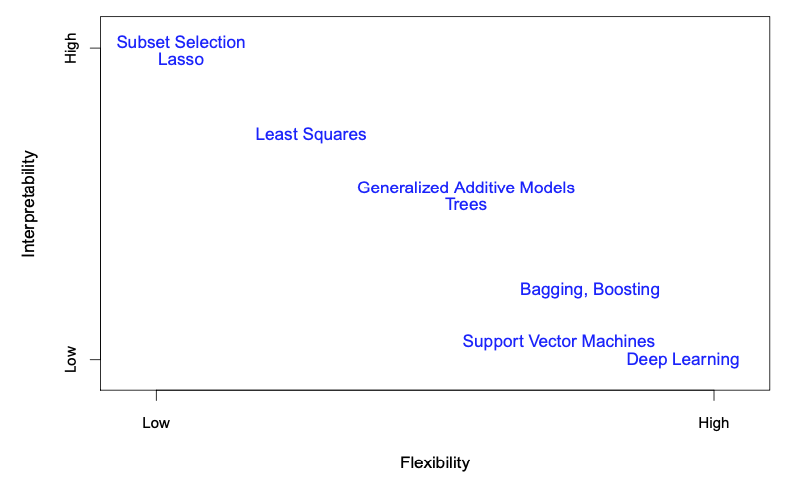
\includegraphics[width=9cm]{data/flexibility}
            };
        }
        \visible<2>{
            \node[] at (0, 1.75) {
                \usebox{\mpglinear}
            };
            \node[] at (0, -1.75) {
                \usebox{\mpgsquared}
            };
        }
        \visible<3>{
            \node[text width=10.5cm, align=flush left] at (0, 0) {
                \textbf{Model performance will depend on the dataset we use to calculate the performance metrics}
                \begin{itemize}
                    \item Training set: The data we use to estimate the model
                    \begin{itemize}
                        \item With a sufficiently flexible model we can \textbf{always} achieve 0 error in the training set
                    \end{itemize}
                    \item Test set: Data held-out from the training set such that it remains unseen by the model
                    \begin{itemize}
                        \item Performance in the test set is indicative of how well the model generalizes to new data (almost always worse than in the training set)
                        \item If our model performs well in new data, we can assume that it accurately describes the relationship between the predictors and the response in the \textbf{general case}
                    \end{itemize}
                \end{itemize}
            };
        }
        \visible<4>{
            \node[text width=10.5cm] at (0, 0) {
                \textbf{How can our model perform poorly?}
                \begin{itemize}
                    \item \underline{Underfitting}: The model is too simple to capture the relationship between the predictors and the response
                    \begin{itemize}
                        \item High error in both the training and test set
                    \end{itemize}
                    \item \underline{Overfitting}: The model is too complex and captures noise in the training set
                    \begin{itemize}
                        \item Low error in the training set, high error in the test set
                    \end{itemize}
                \end{itemize}
            };
        }
        \visible<5>{
            \node[inner sep=0pt, draw=black] at (0, 0) {
                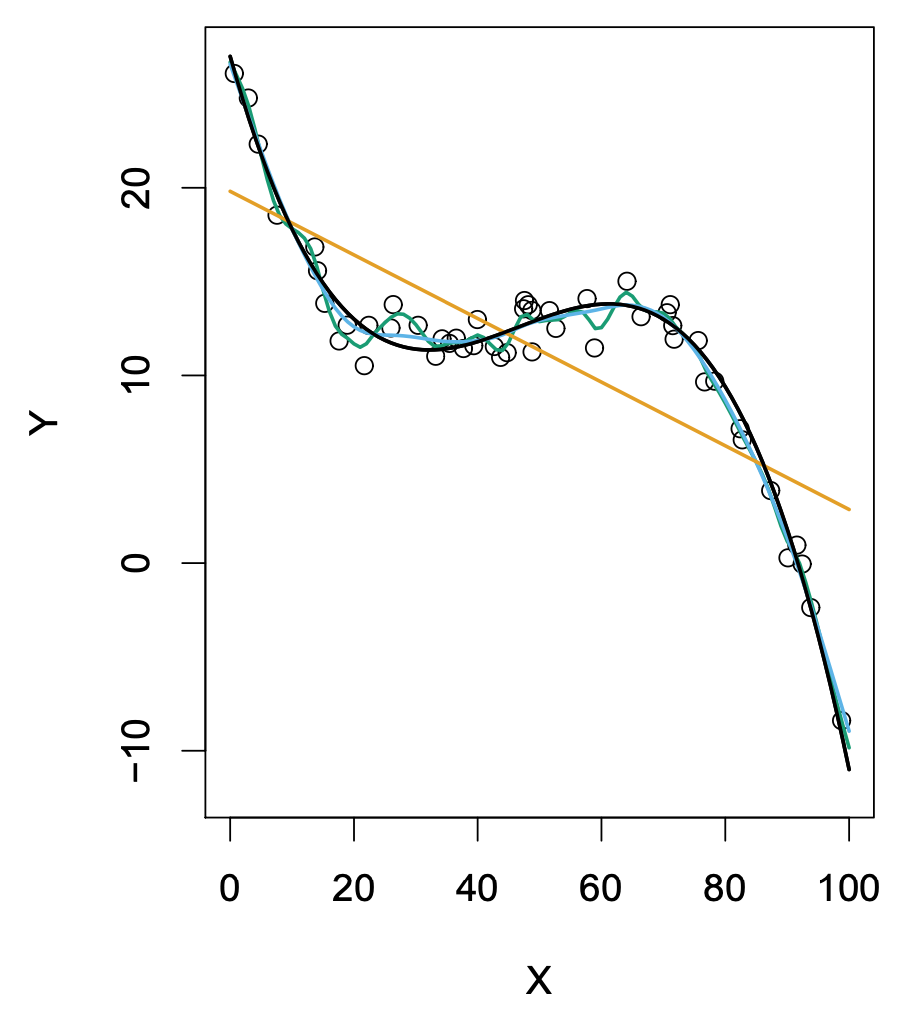
\includegraphics[width=5cm]{data/overfitting_underfitting.png}
            };
        }
        \visible<6-8>{
            \node[] (formula) at (0, 0) {
                $\mathbb{E}\left[\left(y-\hat{f}(x)\right)^2\right]=\mathrm{Var}(\hat{f}(x)) + \left[\mathrm{Bias}(\hat{f}(x))\right]^2+\mathrm{Var}(\epsilon)$
            };
        }
        \visible<7>{
            \node[text=red] (irreducible) at ($ (formula.south) + (3.6, -0.5) $) {
                Irreducible error
            };
            \draw[-stealth, red] (irreducible.north) -- ++(0, 0.5);
        }
        \visible<8>{
            \node[text=red] (bias) at ($ (formula.south) + (1.6, -0.5) $) {
                Bias
            };
            \draw[-stealth, red] (bias.north) -- ++(0, 0.5);

            \node[text=red] (variance) at ($ (formula.south) + (-0.4, -0.5) $) {
                Variance
            };
            \draw[-stealth, red] (variance.north) -- ++(0, 0.5);
        }
        \visible<9-10>{
            \node[] at (-2.675, 1.75) {
                \usebox{\biasvariancetraindata}
            };
        }
        \visible<9-12>{
            \node[font=\footnotesize, text=cyan] at (0, -0.5) {
                $f(x) = -0.000226x^3+0.032262x^2-1.3543x+30+\epsilon$
            };
        }
        \visible<10>{
            \node[] at (2.675, 1.75) {
                \usebox{\biasvariancetestdata}
            };
        }
        \visible<11>{
            \node[] at (-2.675, 1.75) {
                \usebox{\biasvariancetrainlinear}
            };
            \node[] at (2.675, 1.75) {
                \usebox{\biasvariancetestlinear}
            };
        }
        \visible<11-12>{
            \node[font=\footnotesize, text=purple] at (0, -1) {
                $\hat{f}_0(x) = -0.17x+21.74$
            };
        }
        \visible<12-15>{
            \node[] at (-2.675, 1.75) {
                \usebox{\biasvariancetrainpolynomial}
            };
            \node[] at (2.675, 1.75) {
                \usebox{\biasvariancetestpolynomial}
            };
        }
        \visible<12>{
            \node[font=\footnotesize, text=orange] at (0, -1.5) {
                $\hat{f}_1(x) = 1.32*10^{-142}x^{80}-2.18*10^{-140}x^{79}+\ldots$
            };
        }
        \visible<13>{
            \node[] at (-2.675, -1.75) {
                \usebox{\residualtrainlinear}
            };
            \node[] at (2.675, -1.75) {
                \usebox{\residualtestlinear}
            };
        }
        \visible<14>{
            \node[] at (-2.675, -1.75) {
                \usebox{\residualtrainpolynomial}
            };
            \node[] at (2.675, -1.75) {
                \usebox{\residualtestpolynomial}
            };
        }
        \visible<15>{
            \node[] at (-2.675, -1.75) {
                \usebox{\residualtestlinear}
            };
            \node[] at (2.675, -1.75) {
                \usebox{\residualtestpolynomial}
            };
        }
        \visible<16>{
            \node[] at (0, 0.5) {
                \usebox{\tradeoffempty}
            };
        }
        \visible<17>{
            \node[] at (0, 0.5) {
                \usebox{\tradeoffsimple}
            };
        }
        \visible<18>{
            \node[] at (0, 0.5) {
                \usebox{\tradeoffcomplex}
            };
        }
        \visible<19-20>{
            \node[] at (0, 0.5) {
                \usebox{\tradeofftraces}
            };
        }
        \visible<20-21>{
            \node[] (formula) at (0, -2.95) {
                $\mathbb{E}\left[\left(y-\hat{f}(x)\right)^2\right]={\color{variance}\mathrm{Var}(\hat{f}(x))} + {\color{bias}\left[\mathrm{Bias}(\hat{f}(x))\right]^2}+\mathrm{Var}(\epsilon)$
            };
        }
        \visible<21>{
            \node[] at (0, 0.5) {
                \usebox{\tradeoffirreducible}
            };
        }
        \visible<22>{
            \node[] at (0, 0.5) {
                \usebox{\tradeoffloss}
            };
            \node[] (formula) at (0, -2.95) {
                ${\color{full}\mathbb{E}\left[\left(y-\hat{f}(x)\right)^2\right]}={\color{variance}\mathrm{Var}(\hat{f}(x))} + {\color{bias}\left[\mathrm{Bias}(\hat{f}(x))\right]^2}+\mathrm{Var}(\epsilon)$
            };
        }
        \visible<23-24>{
            \node[] at (0, 0.5) {
                \usebox{\tradeofftrain}
            };
        }
        \visible<24>{
            \draw[stealth-stealth, line width=4pt] (-4.6, 0.25) -- (2.7, 0.25);
            \node[font=\bfseries, anchor=north west, draw=black, fill=white, text depth=0] at (-4.6, -0.05) {
                \textbf{Underfitting}
            };
            \node[font=\bfseries, anchor=north east, draw=black, fill=white, text depth=0] at (2.7, -0.05) {
                \textbf{Overfitting}
            };
        }
        \visible<25>{
            \node[text width=10.5cm, align=flush left] at (0, 0) {
                \textbf{The bias-variance trade-off lets us reason about why our model performs poorly}
                \begin{itemize}
                    \item If our model is too simple it will have high bias and low variance, which we can recognize by a high error in both the training and test set
                    \item If our model is too complex it will have low bias and high variance, which we can recognize by a low error in the training set and a high error in the test set
                    \item \textbf{This is way easier in theory than in practice}
                \end{itemize}
            };
        }
    \end{tikzpicture}
\end{frame}

\newsavebox{\groundtruth}
\sbox{\groundtruth}{
    \begin{tikzpicture}
        \begin{axis}[
            height=6cm,
            width=9cm,
            ylabel=$y$,
            xlabel=$x$,
            title style={
                yshift=-0.2cm,
                text depth=0,
            },
            ytick pos=left,
            xtick pos=bottom,
            xmin=0,
            xmax=100
        ]

            \addplot[
                only marks,
                color=cyan,
                opacity=0.25
            ] table [
                col sep=comma,
                x=x,
                y=y
            ] {data/bias-variance-train.csv};
            \addplot[
                very thick,
                domain=-5:105,
                samples=100,
            ] {-0.000226*x*x*x+0.032262*x*x-1.3543*x+30};
        \end{axis}
    \end{tikzpicture}
}

\newcommand{\classificationplot}[1]{
    \begin{tikzpicture}
        \begin{axis}[
            height=6cm,
            width=6cm,
            xlabel=$x_1$,
            ylabel=$x_2$,
            xtick pos=bottom,
            ytick pos=left,
            xmin=-0.99,
            xmax=1.3,
            ymin=-0.65,
            ymax=1.35
        ]
            \ifnum#1=0
                \addplot[
                    only marks,
                    draw=gray,
                    opacity=0.5
                ] table [
                    col sep=comma,
                    x=x1,
                    y=x2
                ] {data/bayesdata.csv};
            \fi

            \ifnum#1>0
                \addplot[
                    only marks,
                    red,
                    opacity=0.5,
                    discard if not={y}{0.0}
                ] table [
                    col sep=comma,
                    x=x1,
                    y=x2
                ] {data/bayesdata.csv};
                \addplot[
                    only marks,
                    blue,
                    opacity=0.5,
                    discard if not={y}{1.0}
                ] table [
                    col sep=comma,
                    x=x1,
                    y=x2
                ] {data/bayesdata.csv};
            \fi

            \ifnum#1=2
                \draw[dashed, thick] (axis cs: -0.6, 1.35) -- (axis cs: 0.8, -0.65);
                \node[anchor=north west, rotate=302, font=\footnotesize\linespread{0.85}\selectfont\bfseries, align=center] at (axis cs: -0.55, 1.35) {
                    Decision\\boundary
                };
            \fi

            \ifnum#1=3
                \addplot [smooth, thick, dashed] coordinates {
                    (-0.3, 1.35)
                    (0.2, 0.2)
                    (0.4, -0.2)
                    (1.6, -0.65)
                };
            \fi
        \end{axis}
    \end{tikzpicture}
}

\newsavebox{\classificationpoints}
\sbox{\classificationpoints}{
    \classificationplot{0}
}
\newsavebox{\classificationclasses}
\sbox{\classificationclasses}{
    \classificationplot{1}
}
\newsavebox{\classificationboundary}
\sbox{\classificationboundary}{
    \classificationplot{2}
}
\newsavebox{\classificationbayes}
\sbox{\classificationbayes}{
    \classificationplot{3}
}

\begin{frame}{Introduction: The Bayes Classifier}
    \begin{tikzpicture}
        \node[] at (-5.25, -3.5) {};
        \node[] at (5.25, 3.5) {};

        \visible<1>{
            \node[] at (0, 0.5) {
                \usebox{\groundtruth}
            };
            \node[] at (0, -2.5) {
                $y=f(x)+\epsilon$
            };
        }
        \visible<2>{
            \node[inner sep=0pt, draw=black, anchor=west] (x1) at (-5.25, 2.5) {
                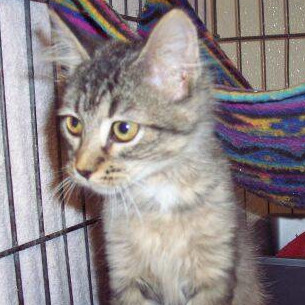
\includegraphics[width=1cm]{data/cats_and_dogs/cat.2.jpg}
            };
            \node[inner sep=0pt, draw=black] (x2) at ($ (x1) - (0, 1.5) $) {
                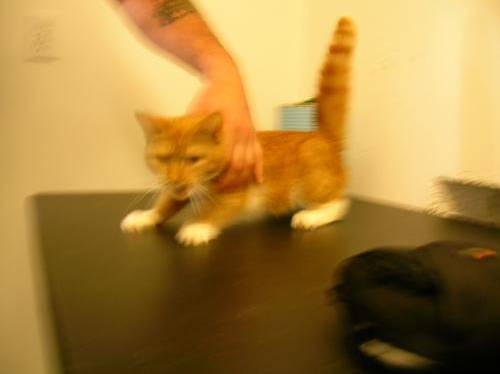
\includegraphics[width=1cm]{data/cats_and_dogs/cat.0.jpg}
            };
            \node[inner sep=0pt, draw=black] (x3) at ($ (x1) - (0, 3) $) {
                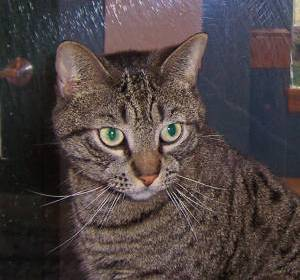
\includegraphics[width=1cm]{data/cats_and_dogs/cat.1.jpg}
            };
            \node[inner sep=0pt, draw=black] (x3) at ($ (x1) - (0, 4.5) $) {
                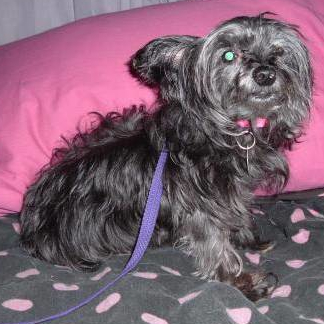
\includegraphics[width=1cm]{data/cats_and_dogs/dog.0.jpg}
            };

            \node[inner sep=0pt, draw=black] (x5) at ($ (x1) - (-1.25, 0.75) $) {
                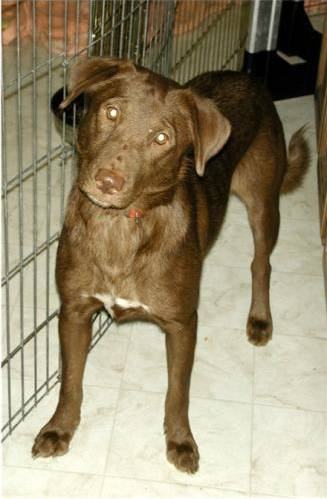
\includegraphics[width=1cm]{data/cats_and_dogs/dog.1.jpg}
            };
            \node[inner sep=0pt, draw=black] (x6) at ($ (x1) - (-1.25, 2.25) $) {
                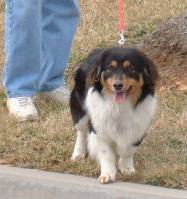
\includegraphics[width=1cm]{data/cats_and_dogs/dog.2.jpg}
            };
            \node[inner sep=0pt, draw=black] (x7) at ($ (x1) - (-1.25, 3.75) $) {
                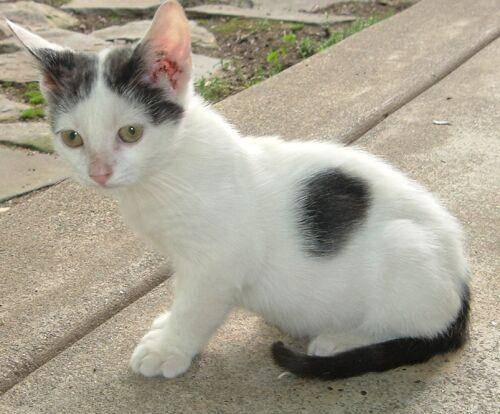
\includegraphics[width=1cm]{data/cats_and_dogs/cat.3.jpg}
            };
            \node[align=center, font=\scriptsize, draw=black] (sm) at ($ (x6) + (2.3, 0) $) {
                Supervised\\model
            };

            \draw[-stealth, gray!50, line width=3pt] (x6) to (sm);
            \draw[-stealth, gray!50, line width=3pt] (sm) -- ($ (sm.east) + (1.1, 0) $);

            \node[inner sep=0pt, draw=black] (y1) at ($ (sm.center) + (5, 0.5) $) {
                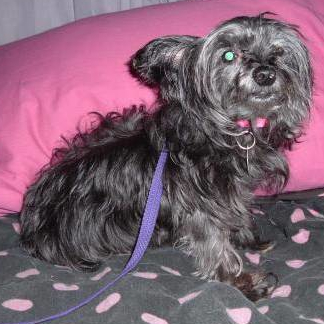
\includegraphics[width=1cm]{data/cats_and_dogs/dog.0.jpg}
            };
            \node[anchor=west, inner sep=0pt, draw=black] (y2) at (y1.east) {
                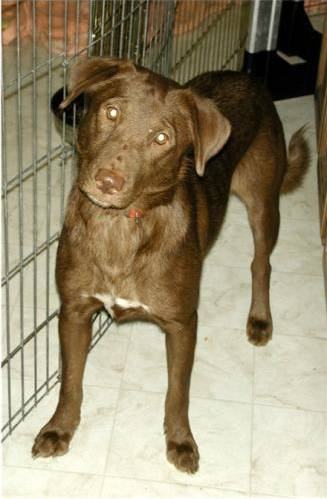
\includegraphics[width=1cm]{data/cats_and_dogs/dog.1.jpg}
            };
            \node[anchor=north, inner sep=0pt, draw=black] at (y1.south) {
                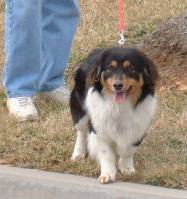
\includegraphics[width=1cm]{data/cats_and_dogs/dog.2.jpg}
            };

            \node[inner sep=0pt, draw=black] (y4) at ($ (sm) + (2.5, 0.5) $) {
                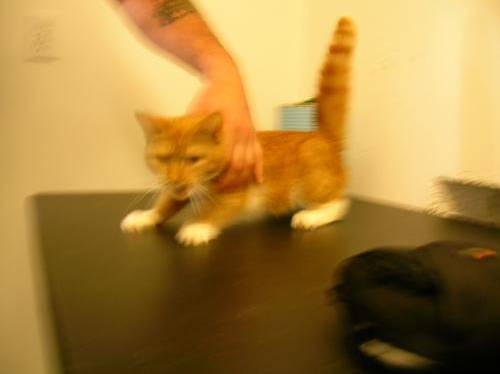
\includegraphics[width=1cm]{data/cats_and_dogs/cat.0.jpg}
            };
            \node[anchor=west, inner sep=0pt, draw=black] (y5) at (y4.east) {
                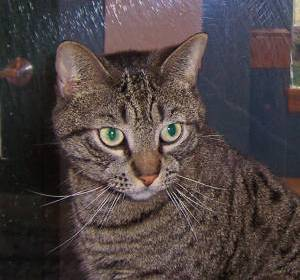
\includegraphics[width=1cm]{data/cats_and_dogs/cat.1.jpg}
            };
            \node[anchor=north, inner sep=0pt, draw=black] (y6) at (y4.south) {
                \includegraphics[width=1cm]{data/cats_and_dogs/cat.2.jpg}
            };
            \node[anchor=north, inner sep=0pt, draw=black] (y7) at (y5.south) {
                \includegraphics[width=1cm]{data/cats_and_dogs/cat.3.jpg}
            };

            \node[anchor=south, text depth=0] at ($ (y1.north)!0.5!(y2.north) $) {
                Dogs
            };
            \node[anchor=south, text depth=0] at ($ (y4.north)!0.5!(y5.north) $) {
                Cats
            };
        }
        \visible<3-7>{
            \node[ampersand replacement=\&] at (-2.75, 0.5) {
                \begin{tabular}{|c|c|c|}
                    \hline
                    $\mathbf{x_1}$&$\mathbf{x_2}$&$\mathbf{y}$\\
                    \hline
                    -0.06&0.17&0\\
                    1.16&1.20&1\\
                    1.12&1.60&1\\
                    0.69&0.28&0\\
                    1.25&1.11&1\\
                    \hline
                \end{tabular}
            };
        }
        \visible<4>{
            \node[] at (2.25, 0.5) {
                \usebox{\classificationpoints}
            };
        }
        \visible<5>{
            \node[] at (2.25, 0.5) {
                \usebox{\classificationclasses}
            };
        }
        \visible<6>{
            \node[] at (2.25, 0.5) {
                \usebox{\classificationboundary}
            };
        }
        \visible<7>{
            \node[] at (2.25, 0.5) {
                \usebox{\classificationbayes}
            };
            \node[] at (2.75, -2.75) {
                $y=\underset{k\in\{0,1\}}{\mathrm{argmax}}\ Pr(y=k|x)$
            };
        }
        \visible<8>{
            \node[text width=10.5cm] at (0, 0) {
                \textbf{Classification can be seen as the task of finding a decision boundary that best separates our classes in a high-dimensional vector space representing our predictors}
                \begin{itemize}
                    \item The Bayes classifier is the best classifier that can be theoretically achieved (although in practice we have to approimate it using data)
                    \item The Bayes error rate quantifies the error of the best possible classifier
                \end{itemize}
            };
        }
    \end{tikzpicture}
\end{frame}

\begin{frame}{Assignment 1}
    Follow the steps in Chapter 2.3 of Introduction to Statistical Learning to make sure your system is set up correctly, whether you want to use Python or R. Then do the following exercises to make sure you understand:

    \begin{itemize}
        \item Create a vector of 100 standard normally distributed numbers and visualize them with a histogram.
        \item Show rows 5, 8, 9, and 10 of the Auto dataset.
        \item Show the last three columns of the Auto dataset.
        \item Show all cars with five cylinders in the Auto dataset.
    \end{itemize}
\end{frame}


    
\newcommand{\mris}[1]{
    \begin{tikzpicture}
        \mriside{0.1}{0}{0.75cm}{0.375}{data/sagittal/0.png}
        \mriside{1.6}{0.1}{0.75cm}{0.375}{data/sagittal/1.png}
        \mriside{3.1}{-0.5}{0.75cm}{0.375}{data/sagittal/2.png}
        \mriside{1.5}{-1.3}{0.75cm}{0.375}{data/sagittal/3.png}
        \mriside{-0.1}{-1.2}{0.75cm}{0.375}{data/sagittal/4.png}

        \mriside{-0.1}{-3.25}{0.75cm}{0.375}{data/sagittal/5.png}
        \mriside{1.35}{-3.4}{0.75cm}{0.375}{data/sagittal/6.png}
        \mriside{3.1}{-3.1}{0.75cm}{0.375}{data/sagittal/7.png}
        \mriside{0.6}{-4.65}{0.75cm}{0.375}{data/sagittal/8.png}
        \mriside{2.3}{-4.7}{0.75cm}{0.375}{data/sagittal/9.png}

        \ifnum#1=1
            \node[font=\footnotesize, text=controls-default] at (1.6, 1) {
                Healthy controls (n=854)
            };
            \node[font=\footnotesize, text=cases-default] at (1.6, -5.6) {
                Dementia patients (n=854)
            };

            \draw[controls-default, dashed] (-0.85, 0.72)
                -- (3.85, 0.72)
                -- (3.85, -1.92)
                -- (-0.85, -1.92)
                -- cycle;
            \draw[cases-default, dashed] (-0.85, -2.48)
                -- (3.85, -2.48)
                -- (3.85, -5.32)
                -- (-0.85, -5.32)
                -- cycle;
        \fi
    \end{tikzpicture}
}

\newcommand{\dataset}{
    \def\legendfont{\footnotesize}

    \begin{tikzpicture}
        \begin{axis}[
            width=0.6\textwidth,
            height=0.8\textwidth,
            xmin=46,
            xmax=99,
            ymin=-1.6,
            ymax=1.2,
            xtick={60,70,80,90},
            axis lines=center,
            axis y line=none,
            clip=false,
            ticklabel style={font=\legendfont}
        ]
            \addplot[name path=zero, draw=none] coordinates {(47,0) (97,0)};

            \addplot[
                name path=fcases,
                draw=cases-default,
                very thick
            ] table [
                col sep=comma,
                x=x,
                y=F-cases
            ]{data/dementia_dataset/dementia_full.csv};\label{trace:cases}
            \addplot[fill=cases-default, opacity=0.2] fill between [of=zero and fcases];

            \addplot[
                name path=fcontrols,
                draw=controls-default,
                very thick
            ] table [
                col sep=comma,
                x=x,
                y=F-controls
            ]{data/dementia_dataset/dementia_full.csv};\label{trace:controls}
            \addplot[fill=controls-default, opacity=0.2] fill between [of=zero and fcontrols];

            \addplot[
                name path=mcases,
                draw=cases-default,
                very thick
            ] table [
                col sep=comma,
                x=x,y
                expr=\thisrow{M-cases} * -1
            ]{data/dementia_dataset/dementia_full.csv};
            \addplot[fill=cases-default, opacity=0.2] fill between [of=zero and mcases];

            \addplot[
                name path=mcontrols,
                draw=controls-default,
                very thick
            ] table [
                col sep=comma,
                x=x,
                y expr=\thisrow{M-controls} * -1
            ]{data/dementia_dataset/dementia_full.csv};
            \addplot[fill=controls-default, opacity=0.2] fill between [of=zero and mcontrols];

            \node[anchor=south west, font=\legendfont] at (axis cs: 43, 0.02) {\textbf{FEMALE}};
            \node[anchor=north west, font=\legendfont] at (axis cs: 43, -0.02) {\textbf{MALE}};
            \node[anchor=south, font=\legendfont, align=center] (n) at (axis cs: 76, -1.2) {\textbf{n=1708}};
        \end{axis}
    \end{tikzpicture}
}

\newcommand{\dementiapredictions}{

    \newcommand{\ymin}{-0.35}
    \newcommand{\ymax}{1.05}

    \begin{tikzpicture}
        \begin{axis}[
            name=distributions,
            height=0.6\textwidth,
            width=9.58cm,
            xtick pos=bottom,
            ymajorticks=false,
            xmajorticks=false,
            xmin=0,
            xmax=1,
            ymin=\ymin,
            ymax=\ymax,
            axis line style={draw=none}
        ]
            \addplot[
                name path=controls,
                draw=controls-default,
                very thick
            ] table [
                col sep=comma,
                x=prediction,
                y=controls
            ]{data/test_distributions.csv};

            \addplot[
                name path=cases,
                draw=cases-default,
                very thick
            ] table [
                col sep=comma,
                x=prediction,
                y=cases
            ]{data/test_distributions.csv};
            \addplot[name path=zero, draw=black] coordinates {(0,0) (1,0)};
            \addplot[fill=controls-default, opacity=0.2] fill between [of=zero and controls];
            \addplot[fill=cases-default, opacity=0.2] fill between [of=zero and cases];
            \addplot[
                scatter/classes={
                    control={controls-default, draw=black, opacity=0.5},
                    case={cases-default, draw=black, opacity=0.5}
                },
                scatter,
                mark=*,
                only marks,
                point meta=explicit symbolic
            ] table [
                col sep=comma,
                y expr=\thisrow{y} * -0.15 - 0.1,
                meta=class,
            ] {data/test_predictions.csv};
        \end{axis}

        \node[anchor=south west] at ($ (distributions.south east) + (0,0.63) $) {\footnotesize{Controls}};
        \node[anchor=south west] at ($ (distributions.south east) + (0,0.12) $) {\footnotesize{Patients}};
    \end{tikzpicture}
}

\begin{frame}{Methodology}
    \begin{tikzpicture}
        \node[draw=black] at (-5.25, -3.5) {};
        \node[draw=black] at (5.25, 3.5) {};

        \only<1>{
            \node[] at (-2.8, 0) {
                \mris{0}
            };
        }
        \only<2-3>{
            \node[] at (-2.8, 0) {
                \mris{1}
            };
        }
        \only<2>{
            \node[] at (2.5, -0.15) {
                \dataset
            };
        }

        \only<3>{
            \node[draw=black, fill=gray, minimum height=2.2cm, minimum width=3.7cm] (model) at (3.2, 0) {};
            \node[minimum height=2.2cm, minimum width=3.7cm, opacity=0.15] at (3.2, 0) {
                \includegraphics[height=2cm]{data/gears.png}
            };
            \node[align=center, minimum height=2.2cm, minimum width=3.7cm, font=\normalfont\linespread{0.9}\bfseries\selectfont, text=white] at (3.2, 0) {
                Machine learning\\model
            };

            \begin{scope}[transparency group, opacity=0.5]
                \draw[-stealth, line width=4pt] (-0.5, 1.65) to [out=0, in=180] ($ (model.west) + (0, 0.22) $);
                \draw[-stealth, line width=4pt] (-0.495, -1.595) to [out=0, in=180] ($ (model.west) - (0, 0.22) $);
            \end{scope}
        }
        \only<5-6>{
            \mriside{-4}{1.45}{1.5cm}{0.75}{data/sagittal/0.png}
            \cnnarrow{(input.east)}{($ (input.center) + (2.5, 0) $)}{black}
        }
        \only<5>{
            \node[anchor=west, font=\small\linespread{0.9}\selectfont, text width=2cm] (healthy) at (3.5, 1.85) {
                Healthy\\control
            };
            \node[anchor=west, text depth=0] (patient) at (3.5, 1.05) {
                Patient
            };

            \cnnarrow{(2.61, 1.45)}{(healthy.west)}{black}
            \cnnarrow{(2.61, 1.45)}{(patient.west)}{black}
        }
        \only<6>{
            \node[anchor=west, text=black!25, font=\small\linespread{0.9}\selectfont, text width=2cm] (healthy) at (3.5, 1.85) {
                Healthy\\control
            };
            \node[anchor=west, text depth=0, font=\small] (patient) at (3.5, 1.05) {
                Patient
            };

            \cnnarrow{(2.61, 1.45)}{(healthy.west)}{black!25}
            \cnnarrow{(2.61, 1.45)}{(patient.west)}{black}
            \node[font=\small\linespread{0.9}\selectfont, align=center, anchor=north] at (-4, 0.25) {
                Healthy\\control
            };
        }
        \only<4-6>{
            \pgfmathsetseed{42}
            \node[] at (0, 1.7) {
                \cnn{0}{0}{0.066}{0.15}{black}{0}{0}
            };
        }

        \only<7-9>{
            \mriside{-4}{1.45}{1.5cm}{0.75}{data/mri_sagittal.png}
            \cnnarrow{(input.east)}{($ (input.center) + (2.5, 0) $)}{black}
            \pgfmathsetseed{43}
            \node[] at (0, 1.7) {
                \cnn{0}{0}{0.066}{0.15}{black}{0}{0}
            };
        }
        \only<7>{
            \node[anchor=west, text width=3cm, font=\small\linespread{0.9}\selectfont] (prediction) at (3.3, 1.45) {
                Predicted\\probability\\of dementia
            };
            \cnnarrow{(2.61, 1.45)}{(prediction.west)}{black}
        }
        \only<8-10>{
            \node[minimum width=8cm, left color=controls-default, right color=cases-default, text=white, draw=black, font=\small\bfseries\selectfont, inner sep=2pt] at (0, -2.75) {Predicted probability of dementia};
            \node[anchor=north] at (-4, -3.02) {0};
            \node[anchor=north] at (0, -3.02) {0.5};
            \node[anchor=north] at (4, -3.02) {1};
        }
        \only<8-9>{
            \node[anchor=west, text width=3cm, font=\small\linespread{0.9}\selectfont] (prediction) at (3.3, 1.45) {
                0.92
            };
            \cnnarrow{(2.61, 1.45)}{(prediction.west)}{black}
            \draw[very thick] (3.36, -3.12) -- (3.36, -2.38);
        }
        \only<9>{
            \node[font=\small] at (-4, 0.1) {
                Patient
            };
            \node[circle, fill=cases-default, draw=black, minimum size=0.14cm, inner sep=0pt, opacity=0.75] at (3.36, -2.2) {};
        }
        \only<10>{
            \node[anchor=south] at (0.576, -2.65) {
                \dementiapredictions
            };
        }
    \end{tikzpicture}
\end{frame}

    \newcommand{\neuron}[3]{
    \node[circle, draw=black, fill=#2] (#1) at #3 {};
}

\begin{frame}{Explainable artificial intelligence}
    \begin{tikzpicture}
        \node[] at (-5.25, -3.5) {};
        \node[] at (5.25, 3.5) {};

        \node[
            draw=black,
            fill=cyan!15,
            minimum height=3cm,
            minimum width=4.3cm,
            label=above:\footnotesize{\textbf{Artificial neural network}}
        ] (model) at (0, 0) {};

        \def\hsep{0.7}
        \def\vsep{0.5}
        \def\edgecolor{gray}
        \def\edgeopacity{0.5}
        \def\neuroncolour{gray}

        \only<1>{
            \neuron{n00}{\neuroncolour}{($ (model) + (-2 * \hsep, -2 * \vsep) $)}
            \neuron{n01}{\neuroncolour}{($ (model) + (-2 * \hsep, -\vsep) $)}
            \neuron{n02}{\neuroncolour}{($ (model) + (-2 * \hsep, 0) $)}
            \neuron{n03}{\neuroncolour}{($ (model) + (-2 * \hsep, \vsep) $)}
            \neuron{n04}{\neuroncolour}{($ (model) + (-2 * \hsep, 2 * \vsep) $)}

            \neuron{n10}{\neuroncolour}{($ (model) + (-\hsep, -1.5 * \vsep) $)}
            \neuron{n11}{\neuroncolour}{($ (model) + (-\hsep, -0.5 * \vsep) $)}
            \neuron{n12}{\neuroncolour}{($ (model) + (-\hsep, 0.5 * \vsep) $)}
            \neuron{n13}{\neuroncolour}{($ (model) + (-\hsep, 1.5 * \vsep) $)}

            \neuron{n20}{\neuroncolour}{($ (model) + (0, -\vsep) $)}
            \neuron{n21}{\neuroncolour}{(model)}
            \neuron{n22}{\neuroncolour}{($ (model) + (0, \vsep) $)}

            \neuron{n30}{\neuroncolour}{($ (model) + (\hsep, -0.5 * \vsep) $)}
            \neuron{n31}{\neuroncolour}{($ (model) + (\hsep, 0.5 * \vsep) $)}

            \neuron{n40}{\neuroncolour}{($ (model) + (2 * \hsep, 0) $)}

            \draw[-stealth, \edgecolor, opacity=\edgeopacity] (model.west) -- (n00);
            \draw[-stealth, \edgecolor, opacity=\edgeopacity] (model.west) -- (n01);
            \draw[-stealth, \edgecolor, opacity=\edgeopacity] (model.west) -- (n02);
            \draw[-stealth, \edgecolor, opacity=\edgeopacity] (model.west) -- (n03);
            \draw[-stealth, \edgecolor, opacity=\edgeopacity] (model.west) -- (n04);

            \foreach \i in {0,...,4} {
                \foreach \j in {0,...,3} {
                    \draw[\edgecolor, opacity=\edgeopacity] (n0\i) -- (n1\j);
                }
            }
            \foreach \i in {0,...,3} {
                \foreach \j in {0,...,2} {
                    \draw[\edgecolor, opacity=\edgeopacity] (n1\i) -- (n2\j);
                }
            }
            \foreach \i in {0,...,2} {
                \foreach \j in {0,...,1} {
                    \draw[\edgecolor, opacity=\edgeopacity] (n2\i) -- (n3\j);
                }
            }
            \foreach \i in {0,...,1} {
                \draw[\edgecolor, opacity=\edgeopacity] (n3\i) -- (n40);
            }

            \draw[-stealth, \edgecolor, opacity=\edgeopacity] (n40) -- (model.east);
        }
        \only<2>{
            \neuron{n00}{black!25}{($ (model) + (-2 * \hsep, -2 * \vsep) $)}
            \neuron{n01}{black!90}{($ (model) + (-2 * \hsep, -\vsep) $)}
            \neuron{n02}{black!72}{($ (model) + (-2 * \hsep, 0) $)}
            \neuron{n03}{black!99}{($ (model) + (-2 * \hsep, \vsep) $)}
            \neuron{n04}{black!10}{($ (model) + (-2 * \hsep, 2 * \vsep) $)}

            \neuron{n10}{black!55}{($ (model) + (-\hsep, -1.5 * \vsep) $)}
            \neuron{n11}{black!92}{($ (model) + (-\hsep, -0.5 * \vsep) $)}
            \neuron{n12}{black!31}{($ (model) + (-\hsep, 0.5 * \vsep) $)}
            \neuron{n13}{black!7}{($ (model) + (-\hsep, 1.5 * \vsep) $)}

            \neuron{n20}{black!50}{($ (model) + (0, -\vsep) $)}
            \neuron{n21}{black!10}{(model)}
            \neuron{n22}{black!100}{($ (model) + (0, \vsep) $)}

            \neuron{n30}{black!75}{($ (model) + (\hsep, -0.5 * \vsep) $)}
            \neuron{n31}{black!65}{($ (model) + (\hsep, 0.5 * \vsep) $)}

            \neuron{n40}{black!95}{($ (model) + (2 * \hsep, 0) $)}

            \draw[-stealth, \edgecolor, opacity=\edgeopacity] (model.west) -- (n00);
            \draw[-stealth, \edgecolor, opacity=\edgeopacity] (model.west) -- (n01);
            \draw[-stealth, \edgecolor, opacity=\edgeopacity] (model.west) -- (n02);
            \draw[-stealth, \edgecolor, opacity=\edgeopacity] (model.west) -- (n03);
            \draw[-stealth, \edgecolor, opacity=\edgeopacity] (model.west) -- (n04);

            \foreach \i in {0,...,4} {
                \foreach \j in {0,...,3} {
                    \draw[\edgecolor, opacity=\edgeopacity] (n0\i) -- (n1\j);
                }
            }
            \foreach \i in {0,...,3} {
                \foreach \j in {0,...,2} {
                    \draw[\edgecolor, opacity=\edgeopacity] (n1\i) -- (n2\j);
                }
            }
            \foreach \i in {0,...,2} {
                \foreach \j in {0,...,1} {
                    \draw[\edgecolor, opacity=\edgeopacity] (n2\i) -- (n3\j);
                }
            }
            \foreach \i in {0,...,1} {
                \draw[\edgecolor, opacity=\edgeopacity] (n3\i) -- (n40);
            }

            \draw[-stealth, \edgecolor, opacity=\edgeopacity] (n40) -- (model.east);

            \node[anchor=east, draw=black, inner sep=0pt] (input) at ($ (model.west) + (-0.77, 0) $) {
                \includegraphics[width=2cm]{data/ladybug.png}
            };
            \cnnarrow{(input.east)}{(model.west)}{black}

            \node[anchor=west] (output) at ($ (model.east) + (0.77, 0) $) {
                Ladybug
            };
            \cnnarrow{(model.east)}{(output.west)}{black}

            \draw[-Latex, line width=3pt] ($ (model.south west) + (0.1, -0.4) $) -- ($ (model.south east) + (-0.1, -0.4) $);

            \node[] at (0, -2.3) {
                \textit{Forward pass}
            };
        }
        \only<3>{
            \neuron{n00}{red!25!black}{($ (model) + (-2 * \hsep, -2 * \vsep) $)}
            \neuron{n01}{red!90!black}{($ (model) + (-2 * \hsep, -\vsep) $)}
            \neuron{n02}{yellow!15!red}{($ (model) + (-2 * \hsep, 0) $)}
            \neuron{n03}{red!99!black}{($ (model) + (-2 * \hsep, \vsep) $)}
            \neuron{n04}{red!10!black}{($ (model) + (-2 * \hsep, 2 * \vsep) $)}

            \neuron{n10}{red!55!black}{($ (model) + (-\hsep, -1.5 * \vsep) $)}
            \neuron{n11}{yellow!20!red}{($ (model) + (-\hsep, -0.5 * \vsep) $)}
            \neuron{n12}{yellow!90!red}{($ (model) + (-\hsep, 0.5 * \vsep) $)}
            \neuron{n13}{red!7!black}{($ (model) + (-\hsep, 1.5 * \vsep) $)}

            \neuron{n20}{red!90!black}{($ (model) + (0, -\vsep) $)}
            \neuron{n21}{red!30!black}{(model)}
            \neuron{n22}{yellow!70!red}{($ (model) + (0, \vsep) $)}

            \neuron{n30}{yellow!40!red}{($ (model) + (\hsep, -0.5 * \vsep) $)}
            \neuron{n31}{red!65!black}{($ (model) + (\hsep, 0.5 * \vsep) $)}

            \neuron{n40}{red}{($ (model) + (2 * \hsep, 0) $)}

            \draw[stealth-, red, opacity=\edgeopacity] (model.west) -- (n00);
            \draw[stealth-, red, opacity=\edgeopacity] (model.west) -- (n01);
            \draw[stealth-, red, opacity=\edgeopacity] (model.west) -- (n02);
            \draw[stealth-, red, opacity=\edgeopacity] (model.west) -- (n03);
            \draw[stealth-, red, opacity=\edgeopacity] (model.west) -- (n04);

            \foreach \i in {0,...,4} {
                \foreach \j in {0,...,3} {
                    \draw[red, opacity=\edgeopacity] (n0\i) -- (n1\j);
                }
            }
            \foreach \i in {0,...,3} {
                \foreach \j in {0,...,2} {
                    \draw[red, opacity=\edgeopacity] (n1\i) -- (n2\j);
                }
            }
            \foreach \i in {0,...,2} {
                \foreach \j in {0,...,1} {
                    \draw[red, opacity=\edgeopacity] (n2\i) -- (n3\j);
                }
            }
            \foreach \i in {0,...,1} {
                \draw[red, opacity=\edgeopacity] (n3\i) -- (n40);
            }

            \draw[stealth-, red, opacity=\edgeopacity] (n40) -- (model.east);

            \node[anchor=east, draw=black, inner sep=0pt] (input) at ($ (model.west) + (-0.77, 0) $) {
                \includegraphics[width=2cm]{data/ladybug_explanation.png}
            };
            \lrparrow{(model.west)}{(input.east)}{red}

            \node[anchor=west, text=red] (output) at ($ (model.east) + (0.77, 0) $) {
                Ladybug
            };
            \lrparrow{(output.west)}{(model.east)}{red}

            \draw[Latex-, line width=3pt, red] ($ (model.south west) + (0.1, -0.4) $) -- ($ (model.south east) + (-0.1, -0.4) $);

            \node[text=red] at (0, -2.3) {
                \textit{Backward pass}
            };
        }
    \end{tikzpicture}
\end{frame}


    \begin{frame}{Explainable AI and dementia}
        \begin{tikzpicture}
            \node[] at (-5.25, -3.5) {};
            \node[] at (5.25, 3.5) {};

            \only<1>{
                \mriside{-4}{-0.25}{1.5cm}{0.75}{data/mri_sagittal.png}
                \cnnarrow{(input.east)}{($ (input.center) + (2.5, 0) $)}{black}
                \pgfmathsetseed{43}
                \node[] at (0, 0) {
                    \cnn{0}{0}{0.066}{0.15}{black}{0}{0}
                };
                \node[anchor=west, text width=3cm, font=\small\linespread{0.9}\selectfont] (prediction) at (3.3, -0.25) {
                    0.92
                };
                \cnnarrow{(2.61, -0.25)}{(prediction.west)}{black}
            }

            \only<2>{
                \mriside{-4}{-0.25}{1.5cm}{0.75}{data/combined_sagittal.png}
                \lrparrow{($ (input.center) + (2.5, 0) $)}{(input.east)}{red}
                \pgfmathsetseed{43}
                \node[] at (0.16, 0) {
                    \lrp{0}{0}{0.066}{0.15}
                };
                \node[anchor=west, text width=3cm, font=\small\linespread{0.9}\selectfont, red] (prediction) at (3.3, -0.25) {
                    0.92
                };
                \lrparrow{(prediction.west)}{(2.61, -0.25)}{red}
            }

            \only<3>{
                \node[
                    minimum height=0.41\textwidth,
                    minimum width=0.32\textwidth,
                    fill=black,
                    anchor=west
                ] (box1) at (-5.25, 0) {};
                \node[anchor=south] at (box1.south) {
                    \includegraphics[width=0.31\textwidth]{data/subject1.png}
                };
                \node[anchor=north,inner sep=2pt, text=white, font=\footnotesize] at (box1.north) {Patient 1};

                \node
                    [minimum height=0.41\textwidth,
                    minimum width=0.32\textwidth,
                    fill=black,
                    anchor=west
                ] (box2) at ($ (box1.east) + (0.05,0) $) {};
                \node[anchor=south] at (box2.south) {
                    \includegraphics[width=0.31\textwidth]{data/subject2.png}
                };
                \node[anchor=north,inner sep=3pt, text=white, font=\footnotesize] at (box2.north) {Partient 2};

                \node
                    [minimum height=0.41\textwidth,
                    minimum width=0.32\textwidth,
                    fill=black,
                    anchor=west
                ] (box3) at ($ (box2.east) + (0.05,0) $) {};
                \node[anchor=south] at (box3.south) {
                    \includegraphics[width=0.31\textwidth]{data/subject3.png}
                };
                \node[anchor=north,inner sep=3pt, text=white, font=\footnotesize] at (box3.north) {Patient 3};
            }
        \end{tikzpicture}
    \end{frame}

    
\begin{frame}{Explainable AI: Caveats}
    \begin{tikzpicture}
        \node[] at (-5.25, -3.5) {};
        \node[] at (5.25, 3.5) {};

        \node[
            draw=black,
            fill=cyan!15,
            minimum height=3cm,
            minimum width=4.3cm,
            label=above:\footnotesize{\textbf{Artificial neural network}}
        ] (model) at (0, 0) {};

        \def\hsep{0.7}
        \def\vsep{0.5}
        \def\edgecolor{gray}
        \def\edgeopacity{0.5}
        \def\neuroncolour{gray}

        \only<1>{
            \neuron{n00}{black!25}{($ (model) + (-2 * \hsep, -2 * \vsep) $)}
            \neuron{n01}{black!90}{($ (model) + (-2 * \hsep, -\vsep) $)}
            \neuron{n02}{black!72}{($ (model) + (-2 * \hsep, 0) $)}
            \neuron{n03}{black!99}{($ (model) + (-2 * \hsep, \vsep) $)}
            \neuron{n04}{black!10}{($ (model) + (-2 * \hsep, 2 * \vsep) $)}

            \neuron{n10}{black!55}{($ (model) + (-\hsep, -1.5 * \vsep) $)}
            \neuron{n11}{black!92}{($ (model) + (-\hsep, -0.5 * \vsep) $)}
            \neuron{n12}{black!31}{($ (model) + (-\hsep, 0.5 * \vsep) $)}
            \neuron{n13}{black!7}{($ (model) + (-\hsep, 1.5 * \vsep) $)}

            \neuron{n20}{black!50}{($ (model) + (0, -\vsep) $)}
            \neuron{n21}{black!10}{(model)}
            \neuron{n22}{black!100}{($ (model) + (0, \vsep) $)}

            \neuron{n30}{black!75}{($ (model) + (\hsep, -0.5 * \vsep) $)}
            \neuron{n31}{black!65}{($ (model) + (\hsep, 0.5 * \vsep) $)}

            \neuron{n40}{black!95}{($ (model) + (2 * \hsep, 0) $)}

            \draw[-stealth, \edgecolor, opacity=\edgeopacity] (model.west) -- (n00);
            \draw[-stealth, \edgecolor, opacity=\edgeopacity] (model.west) -- (n01);
            \draw[-stealth, \edgecolor, opacity=\edgeopacity] (model.west) -- (n02);
            \draw[-stealth, \edgecolor, opacity=\edgeopacity] (model.west) -- (n03);
            \draw[-stealth, \edgecolor, opacity=\edgeopacity] (model.west) -- (n04);

            \foreach \i in {0,...,4} {
                \foreach \j in {0,...,3} {
                    \draw[\edgecolor, opacity=\edgeopacity] (n0\i) -- (n1\j);
                }
            }
            \foreach \i in {0,...,3} {
                \foreach \j in {0,...,2} {
                    \draw[\edgecolor, opacity=\edgeopacity] (n1\i) -- (n2\j);
                }
            }
            \foreach \i in {0,...,2} {
                \foreach \j in {0,...,1} {
                    \draw[\edgecolor, opacity=\edgeopacity] (n2\i) -- (n3\j);
                }
            }
            \foreach \i in {0,...,1} {
                \draw[\edgecolor, opacity=\edgeopacity] (n3\i) -- (n40);
            }

            \draw[-stealth, \edgecolor, opacity=\edgeopacity] (n40) -- (model.east);

            \node[anchor=east, draw=black, inner sep=0pt] (input) at ($ (model.west) + (-0.77, 0) $) {
                \includegraphics[width=2cm]{data/bird.png}
            };
            \cnnarrow{(input.east)}{(model.west)}{black}

            \node[anchor=west] (output) at ($ (model.east) + (0.77, 0) $) {
                Bird
            };
            \cnnarrow{(model.east)}{(output.west)}{black}
        }
        \only<2>{
            \neuron{n00}{red!25!black}{($ (model) + (-2 * \hsep, -2 * \vsep) $)}
            \neuron{n01}{red!90!black}{($ (model) + (-2 * \hsep, -\vsep) $)}
            \neuron{n02}{yellow!15!red}{($ (model) + (-2 * \hsep, 0) $)}
            \neuron{n03}{red!99!black}{($ (model) + (-2 * \hsep, \vsep) $)}
            \neuron{n04}{red!10!black}{($ (model) + (-2 * \hsep, 2 * \vsep) $)}

            \neuron{n10}{red!55!black}{($ (model) + (-\hsep, -1.5 * \vsep) $)}
            \neuron{n11}{yellow!20!red}{($ (model) + (-\hsep, -0.5 * \vsep) $)}
            \neuron{n12}{yellow!90!red}{($ (model) + (-\hsep, 0.5 * \vsep) $)}
            \neuron{n13}{red!7!black}{($ (model) + (-\hsep, 1.5 * \vsep) $)}

            \neuron{n20}{red!90!black}{($ (model) + (0, -\vsep) $)}
            \neuron{n21}{red!30!black}{(model)}
            \neuron{n22}{yellow!70!red}{($ (model) + (0, \vsep) $)}

            \neuron{n30}{yellow!40!red}{($ (model) + (\hsep, -0.5 * \vsep) $)}
            \neuron{n31}{red!65!black}{($ (model) + (\hsep, 0.5 * \vsep) $)}

            \neuron{n40}{red}{($ (model) + (2 * \hsep, 0) $)}

            \draw[stealth-, red, opacity=\edgeopacity] (model.west) -- (n00);
            \draw[stealth-, red, opacity=\edgeopacity] (model.west) -- (n01);
            \draw[stealth-, red, opacity=\edgeopacity] (model.west) -- (n02);
            \draw[stealth-, red, opacity=\edgeopacity] (model.west) -- (n03);
            \draw[stealth-, red, opacity=\edgeopacity] (model.west) -- (n04);

            \foreach \i in {0,...,4} {
                \foreach \j in {0,...,3} {
                    \draw[red, opacity=\edgeopacity] (n0\i) -- (n1\j);
                }
            }
            \foreach \i in {0,...,3} {
                \foreach \j in {0,...,2} {
                    \draw[red, opacity=\edgeopacity] (n1\i) -- (n2\j);
                }
            }
            \foreach \i in {0,...,2} {
                \foreach \j in {0,...,1} {
                    \draw[red, opacity=\edgeopacity] (n2\i) -- (n3\j);
                }
            }
            \foreach \i in {0,...,1} {
                \draw[red, opacity=\edgeopacity] (n3\i) -- (n40);
            }

            \draw[stealth-, red, opacity=\edgeopacity] (n40) -- (model.east);

            \node[anchor=east, draw=black, inner sep=0pt] (input) at ($ (model.west) + (-0.77, 0) $) {
                \includegraphics[width=2cm]{data/edgedetector.png}
            };
            \lrparrow{(model.west)}{(input.east)}{red}

            \node[anchor=west, text=red] (output) at ($ (model.east) + (0.77, 0) $) {
                Bird
            };
            \lrparrow{(output.west)}{(model.east)}{red}
        }
    \end{tikzpicture}
\end{frame}

    \newcommand{\mriwidth}{2.2cm}
\newcommand{\gap}{0.00cm}

\newcommand{\correlationplot}[4]{
    \definecolor{color0}{rgb}{0.62, 0.004, 0.259}
    \definecolor{color1}{rgb}{0.755, 0.154, 0.291}
    \definecolor{color2}{rgb}{0.866, 0.29, 0.298}
    \definecolor{color3}{rgb}{0.943, 0.406, 0.268}
    \definecolor{color4}{rgb}{0.975, 0.557, 0.323}
    \definecolor{color5}{rgb}{0.993, 0.709, 0.403}
    \definecolor{color6}{rgb}{0.995, 0.832, 0.506}
    \definecolor{color7}{rgb}{0.998, 0.926, 0.625}
    \definecolor{color8}{rgb}{0.998, 0.999, 0.746}
    \definecolor{color9}{rgb}{0.937, 0.975, 0.65}
    \definecolor{color10}{rgb}{0.838, 0.935, 0.609}
    \definecolor{color11}{rgb}{0.693, 0.876, 0.639}
    \definecolor{color12}{rgb}{0.527, 0.811, 0.645}
    \definecolor{color13}{rgb}{0.368, 0.725, 0.662}
    \definecolor{color14}{rgb}{0.24, 0.582, 0.721}
    \definecolor{color15}{rgb}{0.267, 0.441, 0.698}
    \definecolor{color16}{rgb}{0.369, 0.31, 0.635}

    \begin{tikzpicture}
        \begin{axis}[
            height=1.715 * \mriwidth,
            width=1.715 * \mriwidth,
            xmajorticks=false,
            ylabel=#3,
            ytick={0, 2, 4, 6, 8},
            yticklabels=#2,
            xmin=-1,
            xmax=17,
            ymin=0,
            ymax=9,
            every tick label/.append style={font=\tiny},
            ytick pos=left,
            scatter/classes={
                ADNI_EF={color0, draw=black},
                ADNI_MEM={color1, draw=black},
                CDCARE={color2, draw=black},
                CDCOMMUN={color3, draw=black},
                CDGLOBAL={color4, draw=black},
                CDHOME={color5, draw=black},
                CDJUDGE={color6, draw=black},
                CDMEMORY={color7, draw=black},
                CDORIENT={color8, draw=black},
                FAQTOTAL={color9, draw=black},
                GDTOTAL={color10, draw=black},
                MMSCORE={color11, draw=black},
                NPISCORE={color12, draw=black},
                PHC_EXF={color13, draw=black},
                PHC_LAN={color14, draw=black},
                PHC_MEM={color15, draw=black},
                PHC_VSP={color16, draw=black}
            },
            y label style={at={(-0.1,0.5)}},
            ymajorgrids=true,
            ytick style={draw=none},
            clip=false,
            grid style={draw=gray!20},
            axis line style={draw=gray!70}
        ]
            \addplot[
                only marks,
                scatter,
                scatter src=explicit symbolic
            ] table [
                col sep=comma,
                x=index,
                y=component_#1,
                meta=symptom
            ] {data/correlations.csv};
            \addplot[dashed,red, thick] coordinates {
                (-1, 2.76)
                (17, 2.76)
            };
            #4
        \end{axis}
    \end{tikzpicture}
}

\newsavebox{\firstcorrelations}
\sbox{\firstcorrelations}{%
    \correlationplot{0}{{0, 2, 4, 6, 8}}{\scriptsize{$-log_{10}(p)$}}{
        \node[] at (axis cs: 14, 6.19) {\tiny{PHC\_LAN}};
    }
}
\newsavebox{\secondcorrelations}
\sbox{\secondcorrelations}{%
    \correlationplot{1}{{,,}}{{}}{
        \node[] at (axis cs: 9, 3.74) {\tiny{FAQTOTAL}};
    }
}
\newsavebox{\thirdcorrelations}
\sbox{\thirdcorrelations}{%
    \correlationplot{2}{{,,}}{{}}{
        \node[] at (axis cs: 0, 6.44) {\tiny{ADNI\_EF}};
        \node[] at (axis cs: 13, 7.95) {\tiny{PHC\_EXF}};
    }
}
\newsavebox{\fourthcorrelations}
\sbox{\fourthcorrelations}{%
    \correlationplot{3}{{,,}}{{}}{
        \node[] at (axis cs: 0, 9.02) {\tiny{ADNI\_EF}};
        \node[] at (axis cs: 13, 8.75) {\tiny{PHC\_EXF}};
        \node[] at (axis cs: 14, 5.84) {\tiny{PHC\_LAN}};
        \node[] at (axis cs: 6, 5.18) {\tiny{CDJUDGE}};
        \node[] at (axis cs: 11, 3.99) {\tiny{MMSCORE}};
    }
}

\newcommand{\cognitivecorrelations}[1]{
    \begin{tikzpicture}
        \node[] at (-1.7, 1.2) {};
        \node[] at (8.7, -5) {};

        \node[] (first) at (0, 0) {
            \includegraphics[
                width=\mriwidth,
                clip=true,
                trim = 192mm 232mm 0mm 0mm
            ]{data/components/component_0.png}
        };

        \node[anchor=west] (second) at ($ (first.east) + (\gap, 0) $) {
            \includegraphics[
                width=\mriwidth,
                clip=true,
                trim = 192mm 232mm 0mm 0mm
            ]{data/components/component_1.png}
        };
        \node[anchor=west] (third) at ($ (second.east) + (\gap, 0) $) {
            \includegraphics[
                width=\mriwidth,
                clip=true,
                trim = 192mm 232mm 0mm 0mm
            ]{data/components/component_2.png}
        };
        \node[anchor=west] (fourth) at ($ (third.east) + (\gap, 0) $) {
            \includegraphics[
                width=\mriwidth,
                clip=true,
                trim = 192mm 232mm 0mm 0mm
            ]{data/components/component_3.png}
        };


        \ifnum#1>0
            \node[anchor=north west] (first-correlation) at ($ (first.south west) + (-0.5, -0.1) $) {
                \hspace{-2.3cm}
                \usebox{\firstcorrelations}
            };
        \fi
        \ifnum#1=2
            \node[anchor=north west] (second-correlation) at ($ (first-correlation.north east) - (0.297, 0) $) {
                \hspace{-2.4cm}
                \usebox{\secondcorrelations}
            };
            \node[anchor=north west] (third-correlation) at ($ (second-correlation.north east) - (0.255, 0) $) {
                \hspace{-2.4cm}
                \usebox{\thirdcorrelations}
            };
            \node[anchor=north west] (fourth-correlation) at ($ (third-correlation.north east) - (0.28, -0.21) $) {
                \hspace{-2.4cm}
                \usebox{\fourthcorrelations}
                \hspace{-0.6cm}
            };
        \fi
    \end{tikzpicture}
}

\newcommand{\prognostic}{
    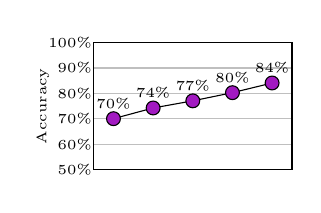
\begin{tikzpicture}
        \begin{axis}[
            height=3.2cm,
            width=4.1cm,
            xmajorticks=false,
            xmin=0.5,
            xmax=5.5,
            ymin=0.5,
            ymax=1,
            ylabel=\tiny{Accuracy},
            ymajorgrids=true,
            ytick={0.5, 0.6, 0.7, 0.8, 0.9, 1},
            yticklabels={50\%, 60\%, 70\%, 80\%, 90\%, 100\%},
            ytick style={draw=none},
            yticklabel style={font=\tiny, xshift=0.1cm},
            ylabel style={yshift=-0.25cm}
        ]
            \addplot[mark=*, draw=black, mark options={fill=additional}, mark size=2.5pt] coordinates {
                (1, 0.701)
                (2, 0.743)
                (3, 0.771)
                (4, 0.803)
                (5, 0.841)
            };
            \node[anchor=south] at (axis cs: 1, 0.701) {\tiny{70\%}};
            \node[anchor=south] at (axis cs: 2, 0.743) {\tiny{74\%}};
            \node[anchor=south] at (axis cs: 3, 0.771) {\tiny{77\%}};
            \node[anchor=south] at (axis cs: 4, 0.803) {\tiny{80\%}};
            \node[anchor=south] at (axis cs: 5, 0.841) {\tiny{84\%}};
        \end{axis}
    \end{tikzpicture}
}

\newsavebox{\prognosticbox}
\sbox{\prognosticbox}{%
    \prognostic
}

\newcommand{\mciconcept}[1]{
    \begin{tikzpicture}
        \begin{axis}[
            height=0.7\textwidth,
            width=0.8\textwidth,
            xlabel={Age},
            ylabel={Cognitive function},
            ticks=none,
            axis x line=bottom,
            axis y line=left,
            y axis line style={-|},
            xmin=0,
            xmax=1.4,
            ymin=0,
            ymax=1,
            clip=false
        ]
            \addplot[draw=healthy-default, smooth, line width=4pt, opacity=0.5] coordinates {
                (0, 0.9)
                (0.25, 0.87)
                (0.5, 0.77)
                (0.6, 0.72)
                (0.8, 0.63)
                (0.9, 0.72)
                (1.4, 0.67)
            };
            \addplot[draw=controls-default, smooth, line width=4pt, opacity=0.5] coordinates {
                (0, 0.9)
                (0.25, 0.87)
                (0.5, 0.77)
                (0.6, 0.72)
                (0.8, 0.63)
                (0.9, 0.61)
                (1.4, 0.54)
            };
            \addplot[draw=cases-default, smooth, line width=4pt, opacity=0.5] coordinates {
                (0, 0.9)
                (0.25, 0.87)
                (0.5, 0.77)
                (0.6, 0.72)
                (0.8, 0.625)
                (1.1, 0.48)
                (1.4, 0.3)
            };
            \addplot[dashed] coordinates {
                (0, 0.65)
                (1.4, 0.65)
            };
            \addplot[dashed] coordinates {
                (0, 0.4)
                (1.4, 0.4)
            };
            \node[anchor=south west] at (axis cs: 0, 0.64) {\footnotesize{Normal cognition}};
            \node[anchor=north west] at (axis cs: 0, 0.66) {\footnotesize{Mild cognitive impairment}};
            \node[anchor=north west] at (axis cs: 0, 0.41) {\footnotesize{Dementia}};

            \node[anchor=west] at (axis cs: 1.4, 0.67) {\textcolor{healthy-default}{\footnotesize{Improving (n=80)}}};
            \node[anchor=west] at (axis cs: 1.4, 0.53) {\textcolor{controls-default}{\footnotesize{Stable (n=754)}}};
            \node[anchor=west] at (axis cs: 1.4, 0.3) {\textcolor{cases-default}{\footnotesize{Progressive (n=354)}}};

            \ifnum#1>0
                \draw[-stealth, red, thick] (axis cs: 0.8, 0.8) -- (axis cs: 0.8, 0.67);
                \node[anchor=south] at (axis cs: 0.8, 0.8) {\textcolor{red}{\footnotesize{t}}};
            \fi

            \ifnum#1>1
                \draw[densely dotted] (axis cs: 0.9, 0.8) -- (axis cs: 0.9, 0.3);
                \draw[densely dotted] (axis cs: 1, 0.8) -- (axis cs: 1, 0.3);
                \draw[densely dotted] (axis cs: 1.1, 0.8) -- (axis cs: 1.1, 0.3);
                \draw[densely dotted] (axis cs: 1.2, 0.8) -- (axis cs: 1.2, 0.3);
                \draw[densely dotted] (axis cs: 1.3, 0.8) -- (axis cs: 1.3, 0.3);
                \node[anchor=south] at (axis cs: 0.9, 0.8) {\footnotesize{t+1}};
                \node[anchor=south] at (axis cs: 1, 0.8) {\footnotesize{t+2}};
                \node[anchor=south] at (axis cs: 1.1, 0.8) {\footnotesize{t+3}};
                \node[anchor=south] at (axis cs: 1.2, 0.8) {\footnotesize{t+4}};
                \node[anchor=south] at (axis cs: 1.3, 0.8) {\footnotesize{t+5}};
            \fi

            \ifnum#1=3
                \node[] at (axis cs: 1.015, 0.162) {
                    \usebox{\prognosticbox}
                };
            \fi

        \end{axis}
    \end{tikzpicture}
}

\begin{frame}{Explainable AI and dementia}
    \begin{tikzpicture}
        \node[] at (-5.25, -3.5) {};
        \node[] at (5.25, 3.5) {};

        \only<1-2>{
            \node[label={[text depth=0]above:Explainable AI}] at (-2.25, 0) {
				\includegraphics[width=0.31\textwidth]{data/dementia.png}
			};
        }
        \only<2>{
			\node[label={[text depth=0]above:Human researchers}] at (2.25, 0) {
				\includegraphics[width=0.31\textwidth]{data/ALE.png}
			};
        }

        \only<3>{
            \node[text width=10cm, font=\scriptsize, align=center] at (0, 0) {
                \renewcommand{\arraystretch}{1.2}
                \begin{tabular}{|>{\centering\arraybackslash}m{2.55cm}|>{\centering\arraybackslash}m{1.45cm}|>{\centering\arraybackslash}m{1.3cm}|>{\centering\arraybackslash}m{2.9cm}|}
                    \hline
                    \textbf{Test battery}&\textbf{Domain}&\textbf{Name}&\textbf{Description}\\
                    \hline
                    Functional Activities Questionnaire&&FAQTOTAL&Measures instrumental activities from everyday life\\
                    \hline
                    ADSP Phenotype Harmonization Consortium&Language&PHC\_LAN&Composite language score\\
                    \hline
                    UW - Neuropsych Summary Scores&Executive functioning&ADNI\_EF&Composite score for executive functioning\\
                    \hline
                    UW - Neuropsych Summary Scores&Memory&ADNI\_MEM&Composite score for memory\\
                    \hline
                \end{tabular}
                \textbf{\vdots}
            };
        }
        \only<4>{
            \node[] at (0.3, 0) {
                \cognitivecorrelations{0}
            };
        }
        \only<5>{
            \node[] at (0.3, 0) {
                \cognitivecorrelations{1}
            };
        }
        \only<6>{
            \node[] at (0.3, 0) {
                \cognitivecorrelations{2}
            };
        }
        \only<7>{
            \node[] at (0, 0) {
                \mciconcept{0}
            };
        }
        \only<8>{
            \node[] at (0, 0) {
                \mciconcept{1}
            };
        }
        \only<9>{
            \node[] at (0, 0) {
                \mciconcept{2}
            };
        }
        \only<10>{
            \node[] at (0, 0) {
                \mciconcept{3}
            };
        }
    \end{tikzpicture}
\end{frame}


    \begin{frame}{Summary}
        We used explainable artificial intelligence to generate heatmaps that characterized the manifestation of dementia in the brains of individual patients.
        \begin{itemize}
            \item The heatmaps focused on brain regions know to be afflicted in dementia
            \item Variability in the heatmaps was associated with neuropsychological variation
            \item The localization of dementia-related aberrations enabled by the heatmaps allowed us to accurately predict progression from mild cognitive impairment to dementia
        \end{itemize}
    \end{frame}
\end{document}
